%% LaTeX2e class for student theses
%% thesis.tex
%% 
%% Karlsruhe Institute of Technology
%% Institute for Program Structures and Data Organization
%% Chair for Software Design and Quality (SDQ)
%%
%% Dr.-Ing. Erik Burger
%% burger@kit.edu
%%
%% See https://sdqweb.ipd.kit.edu/wiki/Dokumentvorlagen
%%
%% {$HeadURL$}
%% {$LastChangedDate$}
%% {$LastChangedRevision$}
%% {$LastChangedBy$}

%% Available page modes: oneside, twoside
%% Available languages: english, ngerman
%% Available modes: draft, final (see README)
\documentclass[twoside, english, draft]{sdqthesis}

%% ---------------------------------
%% | Information about the thesis  |
%% ---------------------------------

%% Name of the author
\author{Yimin Zhang}

%% Title (and possibly subtitle) of the thesis
\title{Interactive Visualization of Correlations in High-Dimensional Streams\\
%	Second Title Line
}

%% Type of the thesis 
\thesistype{Bachelor's Thesis}

%% Change the institute here, ``IPD'' is default
% \myinstitute{Institute for \dots}

%% You can put a logo in the ``logos'' directory and include it here
%% instead of the SDQ logo
% \grouplogo{myfile}
%% Alternatively, you can disable the group logo
 \nogrouplogo

%% The reviewers are the professors that grade your thesis
\reviewerone{Prof. Dr.-Ing. Klemens Böhm}
%\reviewertwo{Prof. B}

%% The advisors are PhDs or Postdocs
\advisorone{M.Sc. Edouard Fouché}
%% The second advisor can be omitted
%\advisortwo{M.Sc. D}

%% Please enter the start end end time of your thesis
\editingtime{01. Mar 2019}{30. Jun 2019}

\settitle

%% --------------------------------
%% | Settings for word separation |
%% --------------------------------

\addto\extrasenglish{%
	\renewcommand{\chapterautorefname}{Chapter}%
	\renewcommand{\sectionautorefname}{Section}%
	\renewcommand{\subsectionautorefname}{Subsection}%
}

%% Describe separation hints here.
%% For more details, see 
%% http://en.wikibooks.org/wiki/LaTeX/Text_Formatting#Hyphenation
\hyphenation{
	% me-ta-mo-del
}

%% --------------------------------
%% | Bibliography                 |
%% --------------------------------
\makeatletter
\DeclareOldFontCommand{\rm}{\normalfont\rmfamily}{\mathrm}
\DeclareOldFontCommand{\sf}{\normalfont\sffamily}{\mathsf}
\DeclareOldFontCommand{\tt}{\normalfont\ttfamily}{\mathtt}
\DeclareOldFontCommand{\bf}{\normalfont\bfseries}{\mathbf}
\DeclareOldFontCommand{\it}{\normalfont\itshape}{\mathit}
\DeclareOldFontCommand{\sl}{\normalfont\slshape}{\@nomath\sl}
\DeclareOldFontCommand{\sc}{\normalfont\scshape}{\@nomath\sc}
\makeatother
%% Use biber instead of BibTeX, see README
%\usepackage[citestyle=numeric,style=numeric,backend=biber]{biblatex}
%\addbibresource{thesis.bib}
\usepackage{subcaption}
%% ====================================
%% ====================================
%% ||                                ||
%% || Beginning of the main document ||
%% ||                                ||
%% ====================================
%% ====================================
\setlength{\parindent}{0pt}
\begin{document}
	
	%% Set PDF metadata
	\setpdf
	
	%% Set the title
	\maketitle
	
	%% The Preamble begins here
	\frontmatter
	
	%% LaTeX2e class for student theses: Declaration of independent work
%% sections/declaration.tex
%% 
%% Karlsruhe Institute of Technology
%% Institute for Program Structures and Data Organization
%% Chair for Software Design and Quality (SDQ)
%%
%% Dr.-Ing. Erik Burger
%% burger@kit.edu
%%
%% Version 1.3.3, 2018-04-17

\thispagestyle{empty}
\null\vfill
\noindent\hbox to \textwidth{\hrulefill} 
\iflanguage{english}{I declare that I have developed and written the enclosed
	thesis completely by myself, and have not used sources or means without
	declaration in the text.}%
{Ich versichere wahrheitsgemäß, die Arbeit
	selbstständig angefertigt, alle benutzten Hilfsmittel vollständig und genau
	angegeben und alles kenntlich gemacht zu haben, was aus Arbeiten anderer
	unverändert oder mit Änderungen entnommen wurde.}


%% ---------------------------------------------
%% | Replace PLACE and DATE with actual values |
%% ---------------------------------------------
\textbf{PLACE, DATE}
\vspace{1.5cm}

\dotfill\hspace*{8.0cm}\\
\hspace*{2cm}(\theauthor) 
\cleardoublepage

	
	\setcounter{page}{1}
	\pagenumbering{roman}
	
	%% ----------------
	%% |   Abstract   |
	%% ----------------
	
	%% For theses written in English, an abstract both in English
	%% and German is mandatory.
	%%
	%% For theses written in German, a German abstract is sufficient.
	%%
	%% The text is included from the following files:
	%% - sections/abstract
	
	\includeabstract
	
	%% ------------------------
	%% |   Table of Contents  |
	%% ------------------------
	\tableofcontents
	
	\listoffigures
	%\listoftables
	
	%% -----------------
	%% |   Main part   |
	%% -----------------
	
	\mainmatter
	
	%% LaTeX2e class for student theses
%% sections/content.tex
%% 
%% Karlsruhe Institute of Technology
%% Institute for Program Structures and Data Organization
%% Chair for Software Design and Quality (SDQ)
%%
%% Dr.-Ing. Erik Burger
%% burger@kit.edu
%%
%% Version 1.3.3, 2018-04-17

\chapter{Introduction}
\label{ch:Introduction}
\section{Motivation}
\label{sec:Introduction:Motivation}
Correlation analysis aims at discovering and summarizing the relationship between the attributes of a data set. Knowing the relationship between a set of variables, one can infer useful knowledge about external, a priori unknown outcomes.\\
For example, we can measure the stock relationship via correlation coefficients in stock markets that may undergo large fluctuations of stock prices. The representing of the correlation coefficients among the five funds’ returns from 1980 to 1998 by Katrina Simons is shown in \autoref{fig:correlations}. Correlation coefficients describe the extent to which asset returns “move together.” Correlation coefficients range in value between negative one (completely negatively correlated) and positive one (completely positively correlated), while a correlation of zero means that there is no correlation between two attributes. Performing good correlation analysis could be of great help to a financial analysis.\\
\begin{figure}[h]
	\centering
	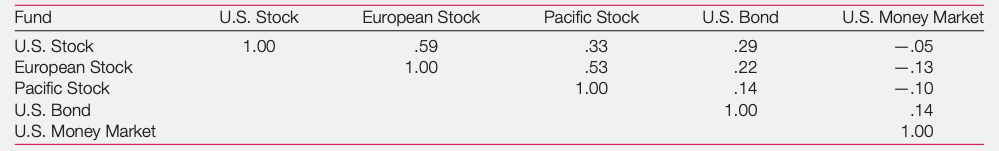
\includegraphics[width=\textwidth]{pictures/motivation1}
	\caption{Correlations Among the Five Funds’ Returns, Monthly Returns, from 1980 to 1998\cite{simons1999should}}
	\label{fig:correlations}
\end{figure}\\
We can see that the stock markets are positive correlated between each other, which indicates a similar behavior during this period. If we are fully aware of our current stock market, we are likely to predict the behavior of other stock markets due to the positive correlation. As a result, if we know that one stock market is performing well, we can maximize our wealth by investing other stock markets, which are positive correlated to our current stock market. If we want to minimize the risk of investing, it's better to invest in no correlated stock markets.
\begin{figure}[h]
	\centering
	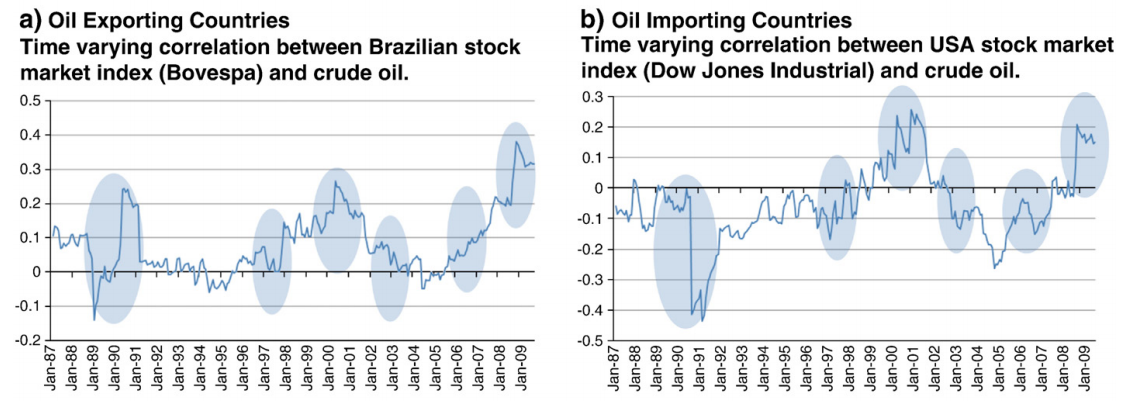
\includegraphics[width=\textwidth]{pictures/motivation21}
	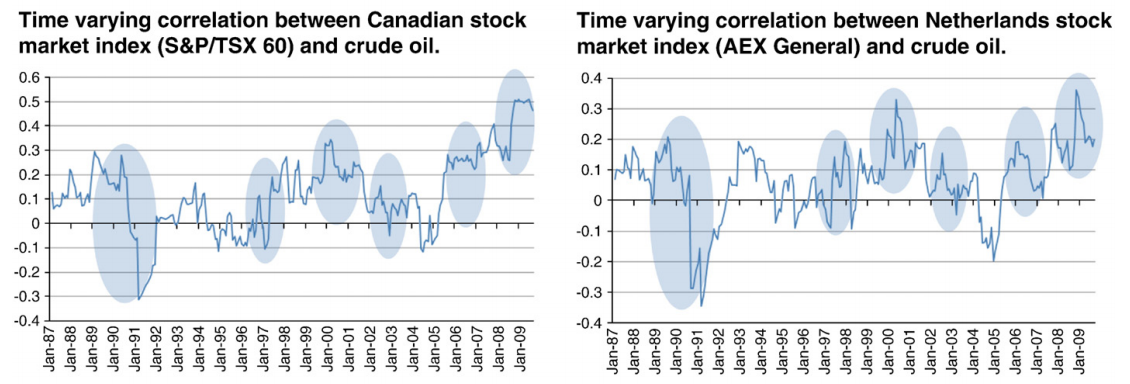
\includegraphics[width=\textwidth]{pictures/motivation22}
	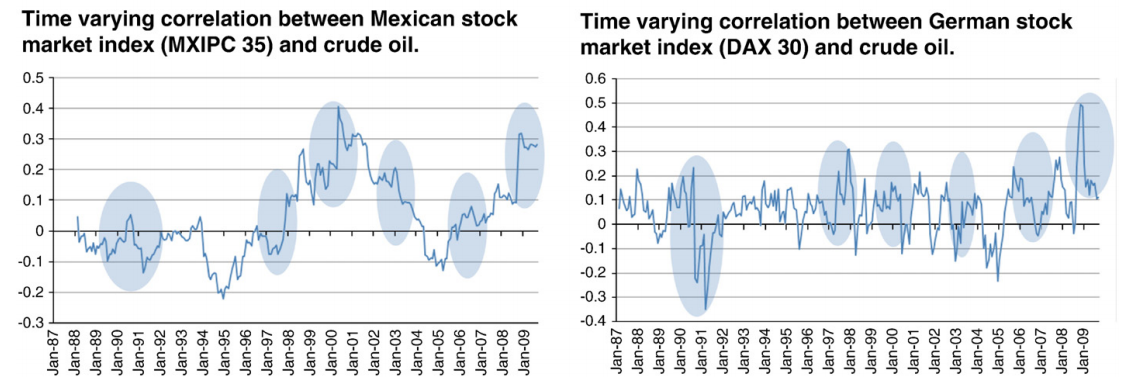
\includegraphics[width=\textwidth]{pictures/motivation23}
	\caption{Dynamic correlation between stock market index and the crude oil price\cite{FILIS2011152}}
	\label{fig:brutal}
\end{figure}\\
Analyzing the correlation between different attributes helps us to understand their relationship. In general, the correlations between attributes remain same or change gradually. If the correlation structure changes brutally, which often indicates a sudden peak or valley, we can infer that one of the attributes may have an enormous change or the relationship between them may differ thoroughly.
George Filis et al. analyzed in \cite{FILIS2011152} the dynamic correlation between stock market index and the crude oil price, which is shown in \autoref{fig:brutal}. During the period 1987 - 2009, 6 important events occurred: 
\begin{itemize}
	\item Iraq invasion in Kuwait/first war in Iraq
	\item Asian economic crisis
	\item Housing market boom
	\item Second war in Iraq
	\item Chinese economic growth
	\item Global financial crisis
\end{itemize}
These events signed the brutal changes in the correlation between markets and oil price, which are printed in blue circles in the \autoref{fig:brutal}.\\

\section{Challenges}
\label{sec:Introduction:Challenges}
The challenges of analyzing high-dimensional data streams is twofold: the evolving nature of streams and the high-dimensionality.\\

\subsection{The evolving nature of streams}
\label{sec:Introduction:Challenges:Streams}
In contrast to static data, the data is often available as a stream, i.e., it is an infinite, ever evolving sequence of observations. As the concepts learned at a certain time cannot be expected to hold in the future, correlation analysis should be a continuous process. We can see from \autoref{fig:brutal} that the correlation between market and oil price is always changing throughout the time. The correlation values even have brutal changes, when meet up with important events. Therefore, it's quite hard for the data scientists to predict the correlation value at next timestamp.\\

\subsection{The high-dimensionality}
\label{sec:Introduction:Challenges:High-dimensionality}
Also, the data is often high-dimensional, i.e., it contains hundreds or thousands of dimensions. In the case of streams with many dimensions, it is difficult to extract actionable insights from the correlation matrix, as the number of pairs of attributes increases quadratically and the coefficients evolve over time in unforeseen ways. For the pairwise correlation analysis of any data steam with $n$ components, one need to compute the correlation between $ \dfrac{n*(n-1)}{2} $ pairs, i.e., with $ n=5 $, one needs to compute 10 pairs, with $ n=10 $, one needs to compute 45 pairs. Therefore, it becomes difficult to visually keep track of correlation and impossible to understand the result of the correlation analysis as the number of attributes increases. The \autoref{fig:visualization} shows the visualization of different numbers of attributes. As an instance, with the developing number of attributes, it becomes even harder for users to compare the correlation value between two pairs using Heatmap as the standard tool to visualize the data.\\
\begin{figure}[h]
	\centering
\begin{subfigure}[b]{0.3\textwidth}
	\centering
	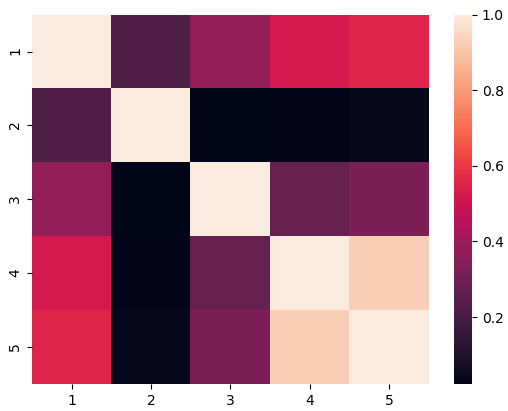
\includegraphics[width=\textwidth]{pictures/bioliq5}
	\caption{Correlation matrix of 5 attributes}
	\label{fig:matrix5}
\end{subfigure}
\hfill
\begin{subfigure}[b]{0.3\textwidth}
	\centering
	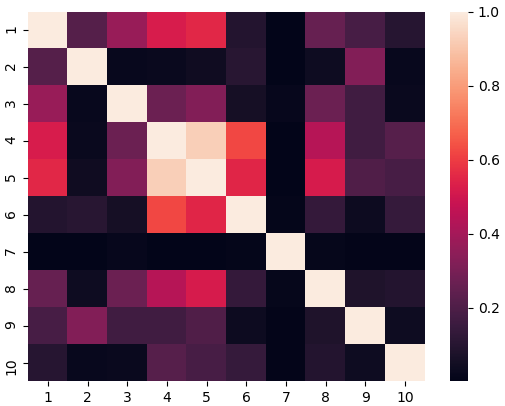
\includegraphics[width=\textwidth]{pictures/bioliq10}
	\caption{Correlation matrix of 10 attributes}
	\label{fig:matrix10}
\end{subfigure}
\hfill
\begin{subfigure}[b]{0.3\textwidth}
	\centering
	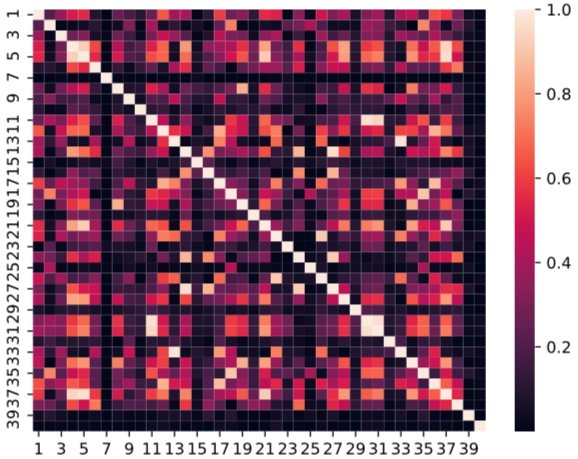
\includegraphics[width=\textwidth]{pictures/bioliq40}
	\caption{Correlation matrix of 40 attributes}
	\label{fig:matrix40}
\end{subfigure}
	\caption{Visualizations of different numbers of attributes}
	\label{fig:visualization}
\end{figure}
\section{Goal of the thesis}
\label{sec:Introduction:GoalOfTheThesis}
The goal of this thesis is to propose and evaluate new tools for the interactive visualization of correlation in high-dimensional streams. We are going to compare different visualization methods. Our interactive interface aims at providing a visualization of correlations in streams, which may change arbitrarily over time, for people. Users are able to choose a certain period of time to perform the correlation analysis and visualization. In our thesis, we only focus on pairwise relationships and the correlations between more than two variables may remain to be discovered in the future work. We are going to answer the following three questions in the thesis:
\begin{itemize}
	\item What visualization method is the most appropriate to visualize correlation for various specific user information needs?
	\item What visualization method is the most suitable to visualize characteristics of a data set?
	\item What are the desirable features of a correlation monitoring interface?
\end{itemize}
To answer these questions, we first search for three interactive visualization methods and then develop an interface to visualize correlations using these methods. This interface can be available in a browser and should be user friendly, which means that users provide their own data sets and the system’s back-end calculates the correlations and then provides the visualization of the results. Users are also able to interact in several ways with this interface, such as setting parameters to tune the visualization. At last, we evaluate the benefits of our interface systematically via controlled user studies and discuss the advantages and disadvantages of each visualization method when meet up with different scenarios. Based on the results, we discover the appropriate visualization methods of correlations in high-dimensional streams and the desirable features of the interactive interface.\\
\section{Thesis outline}
\label{sec:Introduction:ThesisOutline}
This thesis is divided into three parts: the literature review of visualization methods, the design and implementation of interface, and the evaluation of this interface.\\
In \autoref{ch:Visualization}, the first part of the thesis, we introduce three state-of-art methods for correlation visualization: Heatmap, Bar Graph and Force-Directed-Graph.\\
\autoref{ch:RelatedWork} is about the related work. In \autoref{ch:RelatedWork}, we give an overview\cite{Matrics} of parallel coordinates and scatterplot matrices as examples of multidimensional visualization techniques. Also, we introduce an interactive Framework for Exploring and Understanding Multivariate Correlations "FEXUM"\cite{FEXUM} created by Louis Kirsch et al., which uses Force-Directed-Graph as the visualization method for the data set.\\
\autoref{ch:Interface} is the main part of this thesis. \autoref{sec:Interface:Design} is the design of the interface and \autoref{sec:Interface:Implementation} describes the implementation of this interface.\\
We evaluate the developed interface in \autoref{ch:Evaluation}. It contains not only the experimental settings of controlled user studies for evaluation in \autoref{sec:Evaluation:ExperimentalSettings}, but also the results of controlled user studies and feedbacks in \autoref{sec:Evaluation:Result}.\\
The summary of the whole thesis comes in the end.\\
	%% LaTeX2e class for student theses
%% sections/content.tex
%% 
%% Karlsruhe Institute of Technology
%% Institute for Program Structures and Data Organization
%% Chair for Software Design and Quality (SDQ)
%%
%% Dr.-Ing. Erik Burger
%% burger@kit.edu
%%
%% Version 1.3.3, 2018-04-17

\chapter{Visualization Methods}
\label{ch:Visualization}
In this chapter, we first introduce the correlation matrix in \autoref{sec:Visualization:CorrelationMatrix} and then introduce three useful interactive visualization methods \autoref{sec:Visualization:Heatmap} Heatmap, \autoref{sec:Visualization:BarGraph} Bar Graph and \autoref{sec:Visualization:ForceDirectedGraph} Force-Directed-Graph, and give examples of each visualization method using the same data set in \autoref{sec:Visualization:mtcars}.\\

\section{Correlation Matrix}
\label{sec:Visualization:CorrelationMatrix}
The most familiar measure of dependence between two quantities is the Pearson product-moment correlation coefficient\cite{correlation}, known as "Pearson's correlation coefficient". It is obtained by dividing the covariance of the two variables by the product of their standard deviations. The population correlation coefficient $\rho _{X,Y}$ between two random variables $X$ and $Y$ and standard deviations $\sigma _{X}$ and $\sigma_Y$ is defined as
\begin{equation}
\rho _{X,Y}=\operatorname {corr} (X,Y)={\operatorname {cov} (X,Y) \over \sigma _{X}\sigma _{Y}}
\end{equation}
where $\operatorname {cov}$ means covariance, and $\operatorname {corr}$ is a widely used alternative notation for the correlation coefficient. The Pearson correlation is defined only if both of the standard deviations are finite and non-zero.\\
The standard tool of correlation analysis is the computation of a correlation matrix
\begin{equation}
\rho = \begin{bmatrix}
	\rho_{1,1} & \dots & \rho_{1,n} \\ 
	\dots & \dots & \dots \\ 
	\rho_{n,1} & \dots & \rho_{n,n}
\end{bmatrix}
n \in \mathcal{N}^*
\end{equation}
for n variables. The correlation matrix is used to investigate the dependence between multiple variables at the same time. In fact, we are only interested in the lower half of the matrix because of its symmetry and invariant diagonal line.\\

\section{Data Set Mtcars}
\label{sec:Visualization:mtcars}
Data Set Mtcars represents Auto MPG Data Set, which can be found in UCI Machine Learning Repository by url: https://archive.ics.uci.edu/ml/datasets/auto+mpg. It is a data frame with 32 observations on 11 variables. This data set can be seen as a standard data set widely-used in the field of data analysis. \autoref{sec:Visualization:Heatmap}, \autoref{sec:Visualization:BarGraph} and \autoref{sec:Visualization:ForceDirectedGraph} all use this data set to visualize.

\section{Heatmap}
\label{sec:Visualization:Heatmap}
A common visualization is the heatmap\cite{heatmap}, which is originated in 2D displays of the values in a data matrix. The \autoref{fig:Heatmap} is a heatmap of a correlation matrix, in which the variables with strong correlation (high values) are printed in light colour and those with low correlation are in dark colour.\\

\section{Bar Graph}
\label{sec:Visualization:BarGraph}
A bar graph\cite{bar} presents categorical data with rectangular bars with heights or lengths proportional to the values that they represent. We use vertical bar graph in our developed interface. In a vertical bar graph, the x-Axis shows the specific categories being compared, and the y-Axis represents a measured value, which is the correlation value in our situation. Bar graphs provide a visual presentation of categorical data, which are usually qualitative. \autoref{fig:Bar Graph} is a bar graph, using the same data set in \autoref{fig:Heatmap}.\\

\section{Force-Directed-Graph}
\label{sec:Visualization:ForceDirectedGraph}
Force-Directed-Graph\cite{force} assigns forces among the set of edges and the set of nodes of a graph drawing. The purpose of it is to position the nodes of a graph in two-dimensional or three-dimensional space so that all the edges are of more or less equal length and there are as few crossing edges as possible. In such a simulation, the forces are applied to the nodes, pulling them closer together or pushing them further apart. This can be used to simulate the relationship of different attributes throughout the time. \autoref{fig:Force-Directed-Graph} is the example of Force-Directed-Graph, which also uses Data Set Mtcars.\\
\begin{figure}[h]
	\centering
	\begin{subfigure}[b]{0.32\textwidth}
		\centering
		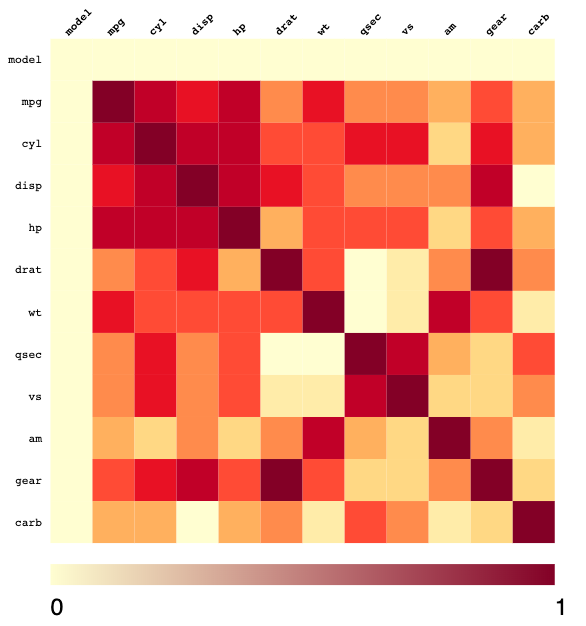
\includegraphics[width=\textwidth]{pictures/correlationMatrix}
		\caption{Heatmap as the visualization method}
		\label{fig:Heatmap}
	\end{subfigure}
	\hfill
	\begin{subfigure}[b]{0.32\textwidth}
		\centering
		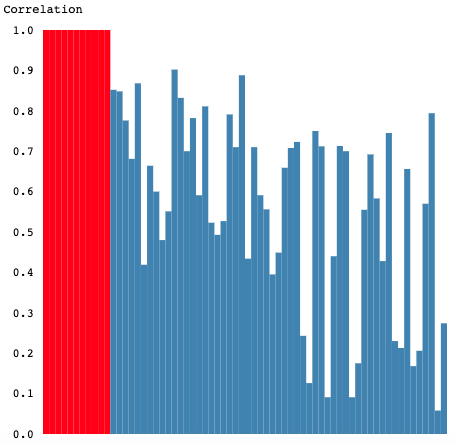
\includegraphics[width=\textwidth]{pictures/bg}
		\caption{Bar Graph as the visualization method}
		\label{fig:Bar Graph}
	\end{subfigure}
	\hfill
	\begin{subfigure}[b]{0.32\textwidth}
		\centering
		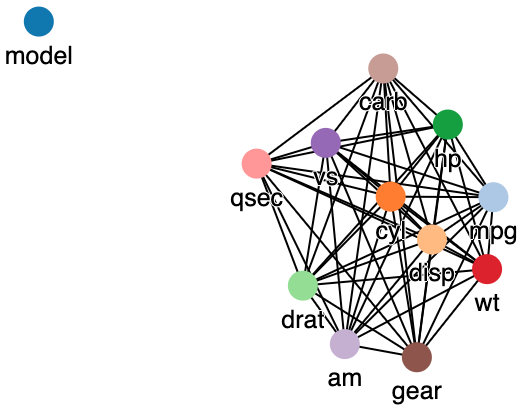
\includegraphics[width=\textwidth]{pictures/fdg}
		\caption{Force-Directed-Graph as the visualization method}
		\label{fig:Force-Directed-Graph}
	\end{subfigure}
	\caption{Three visualization methods of the Data Set Mtcars}
	\label{fig:vis}
\end{figure}

	%% LaTeX2e class for student theses
%% sections/content.tex
%% 
%% Karlsruhe Institute of Technology
%% Institute for Program Structures and Data Organization
%% Chair for Software Design and Quality (SDQ)
%%
%% Dr.-Ing. Erik Burger
%% burger@kit.edu
%%
%% Version 1.3.3, 2018-04-17

\chapter{Related Work}
\label{ch:RelatedWork}
With the exponentially increasing amount of acquired multivariate data, several multi-dimensional visualization techniques have been proposed during the last decades. Parallel coordinates and scatterplot matrices are widely used to visualize multi-dimensional data sets. But these visualization techniques are insufficient when the number of dimensions grows. To solve this problem, different approaches to select the best views or dimensions in advance have been proposed in the last years.\\ 
\begin{figure}[h]
	\centering
	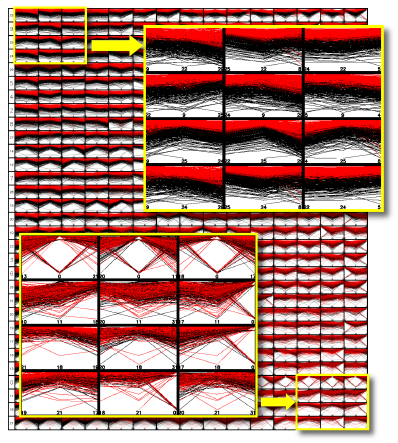
\includegraphics[width=0.4\textwidth]{pictures/PCM}
	\caption{Parallel coordinates matrices\cite{Matrics} for the data set}
	\label{fig:PCM}
\end{figure}
\\Georgia Albuquerque et al. presented three new methods to explore multivariate data sets: a parallel coordinates matrix (\autoref{fig:PCM}), in analogy to the well-known scatterplot matrix, a class-based scatterplot matrix that aims at finding good projections for each class pair (\autoref{fig:C-SPLOM}), and an importance aware algorithm\cite{Matrics} to sort the dimensions of scatterplot and parallel coordinates matrices. They aims at providing a visualization of the whole data set, not the correlations of attributes in this data set. As we focus on the correlations only between each two attributes in our thesis, it is no need for us to have parallel coordinates in our framework.
\begin{figure}[h]
	\centering
	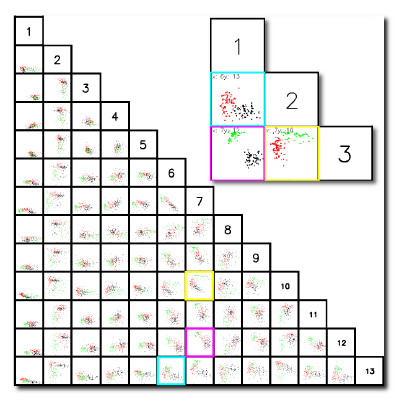
\includegraphics[width=0.4\textwidth]{pictures/C-SPLOM}
	\caption{Class-based scatterplot matrices\cite{Matrics} for the data set}
	\label{fig:C-SPLOM}
\end{figure}
\\In \autoref{sec:Introduction:Motivation}, we have pointed out the use and importance of correlation analysis between different attributes, which helps people to understand the relationship of attributes in a data set. Unlike the work of Georgia Albuquerque et al.\cite{Matrics}, our interface provides the visualization of correlation values in a data set.\\
As a high-dimensional data set may contain many redundant features, feature selection becomes an essential step for correlation analysis. Louis Kirsch et al. developed an interactive Framework for Exploring and Understanding Multivariate Correlations (FEXUM)\cite{FEXUM} to simultaneously visualize all feature correlations to the target and pairwise correlations using Force-Directed-Graph. This visualization provides a layout in which a smaller distance between two features denotes a greater redundancy. In \autoref{fig:FEXUM}, nodes represent features and weighted edges represent distances. FEXUM provides users with an understanding of how features interact with each other in terms of redundancy so that they can easily find influential value ranges in the analysis view and make feature selection.\\
In our developed interface, we give the users an overview of all correlations in the data set. Instead of choosing a target attribute to focus on, our system represents the whole correlations of the data set. Unlike FEXUM\cite{FEXUM}, Force-Directed-Graph is not the only visualization method in our system. Heat map and Bar graphs are alternative visualization method for the users so that the users can choose the most suitable visualization method in their opinion.\\
In \autoref{sec:Introduction:Challenges:Streams}, we have discussed that the correlation analysis should be a continuous process. FEXUM enables the users to upload their own data sets and visualize them. However, in our system, the uploaded data set by users can be a data set of data stream so that the users can choose a period of time to perform the correlation analysis and visualization. Our goal is to visualize a concise but useful summary of correlations in the stream over time.\\
\begin{figure}[h]
	\centering
	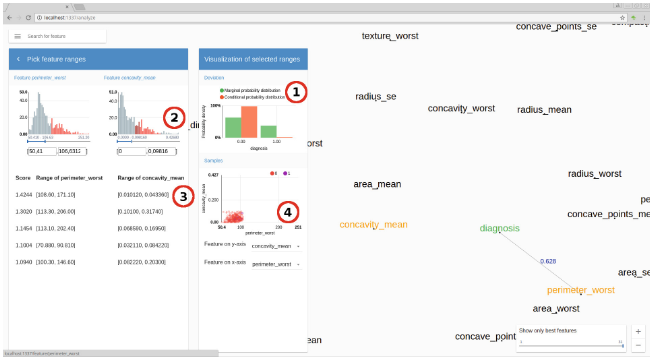
\includegraphics[width=\textwidth]{pictures/FEXUM}
	\caption{Features drawn using a force-directed graph (right), with the target highlighted in green. An analysis view of two features (left) for inspecting the correlations.\cite{FEXUM}}
	\label{fig:FEXUM}
\end{figure}
	%% LaTeX2e class for student theses
%% sections/content.tex
%% 
%% Karlsruhe Institute of Technology
%% Institute for Program Structures and Data Organization
%% Chair for Software Design and Quality (SDQ)
%%
%% Dr.-Ing. Erik Burger
%% burger@kit.edu
%%
%% Version 1.3.3, 2018-04-17

\chapter{Interface}
\label{ch:Interface}
To answer the questions we mentioned in the \autoref{sec:Introduction:GoalOfTheThesis}, we develop an interface in a browser available as a web-service. The entire framework is open source and available online via url https://github.com/yimin95/InteractiveVisualization. In \autoref{sec:Interface:Design}, we describe the mock-up of this interface and its available functions. And we introduce the details of implementation in \autoref{sec:Interface:Implementation}.\\

\section{Design}
\label{sec:Interface:Design}
\autoref{fig:mockup} is the mock-up of this interface. This interface can be used with a wide range of data sets as csv files, supplied through upload by the user. The first line of such file is the list of attributes' names. The corresponding values of each attributes are displayed in the following lines. The following table is an example of a csv file, while the blanking blocks are values of corresponding attributes.\\
	\begin{tabular}{ | l | l | l | l | l | l |}
		\hline
		Attribute 1 & Attribute 2 & Attribute 3 & Attribute 4 & Attribute 5 & Attribute 6 \\ \hline
		            &             &             &             &             &             \\ \hline
		            &             &             &             &             &             \\ \hline
		            &             &             &             &             &             \\ \hline
	\end{tabular}
\\\\After the calculation in the back-end, the visualization of data correlation is shown in the website, for example, via a Heatmap. In the mock-up, a sliding window with start point and step size is supposed to be used to represent the continuous process of data throughout the time. Also, we have some simple user settings, such as changing the window size, setting the minimum and maximum of correlation to be visualized.\\
In our interface, we focus on the absolute value of the correlation. \textbf{Minimum} is the minimal value of the correlation value and it is set to 0 as default. \textbf{Maximum} is the maximal value of the correlation value and it is set to 1 as default. \textbf{The window size} represents the size of the selected timestamps of the current data set. Timestamp represents the instance of data set. As we aim at data stream, each instance of data set is the representation for values of attributes at a certain timestamp. The width of panel on the slider indicates the size of the current window. With the sliding of panel, visualizations of correlations during different time periods are shown on the website, representing the visualization of correlation in data streams. \textbf{the step size} gives out the difference between two adjacent movements of slider. Combined with the step size, the user is able to get the visualization of a certain time period by sliding the sliding window. \textbf{The current point} represents the starting point of current selected group of timestamps. It is also possible for the user to input the starting point of timestamps.\\

\begin{figure}[h]
	\centering
	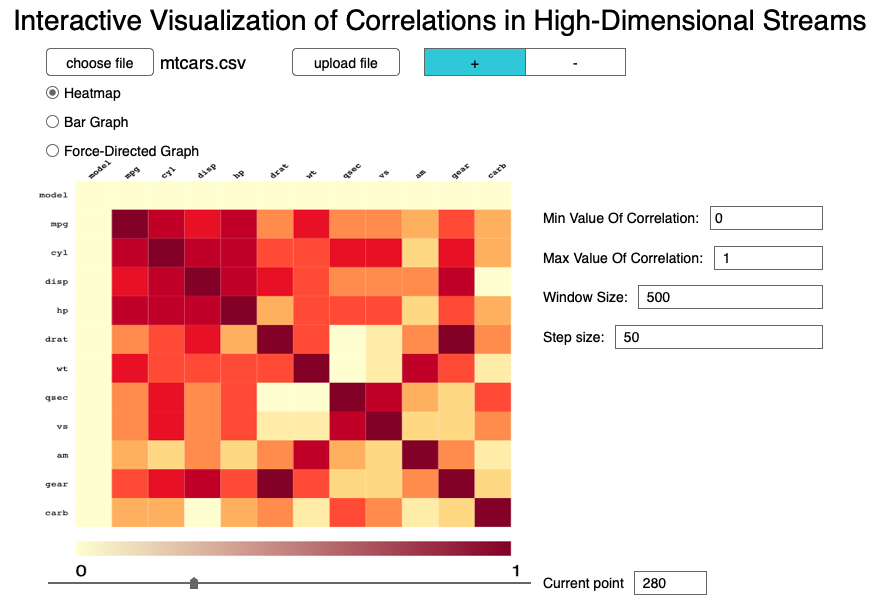
\includegraphics[width=15cm]{pictures/mockup}
	\caption{Mock-up of the interface}
	\label{fig:mockup}
\end{figure}

\section{Implementation}
\label{sec:Interface:Implementation}
As the interface is available by the web service, Javascript is the programming language for developing. In our project, we mainly use D3.js to implement the visualizations of correlations in high-dimensional data streams.
\subsection{D3.js}
\label{sec:Visualization:D3.js}
D3.js (Data-Driven Documents)\cite{D3} is a data-driven JavaScript library for producing dynamic, interactive data visualizations in web browsers. It makes use of the widely implemented SVG, HTML5, and CSS standards and allows great control over the final visual result. SVG stands for Scalable Vector Graphics which is technically an XML based markup language. It is a great tool to display icons, logos, illustrations or charts, which is supported in all major browsers and requires no third-party lib because of owning the DOM interface.\\

%What is D3.js?
%D3.js is a data-driven JavaScript library for manipulating DOM elements.
%“D3 helps you bring data to life using HTML, SVG, and CSS. D3’s emphasis on web standards gives you the full capabilities of modern browsers without tying yourself to a proprietary framework, combining powerful visualization components and a data-driven approach to DOM manipulation.” - d3js.org

%Why would You create charts with D3.js in the first place? Why not just display an image?

%Well, charts are based on information coming from third-party resources which requires dynamic visualization during render time. Also, SVG is a very powerful tool which fits well to this application case.

%The benefits of SVG
%SVG stands for Scalable Vector Graphics which is technically an XML based markup language.
%It is commonly used to draw vector graphics, specify lines and shapes or modify existing images. You can find the list of available elements here.

%Pros:
%Supported in all major browsers;
%It has DOM interface, requires no third-party lib;
%Scalable, it can maintain high resolution;
%Reduced size compared to other image formats.

%Cons:
%It can only display two-dimensional images;
%Long learning curve;
%Render may take long with compute-intensive operations.
%Despite its downsides, SVG is a great tool to display icons, logos, illustrations or in this case, charts.

\subsection{Details}
\label{sec:Visualization:Details}
The \autoref{fig:overview} is an overview of our developed interface, which is available in a browser as a web-service. Users can press the "Choose file" button to upload their own data sets.\\

\begin{figure}[h]
	\centering
	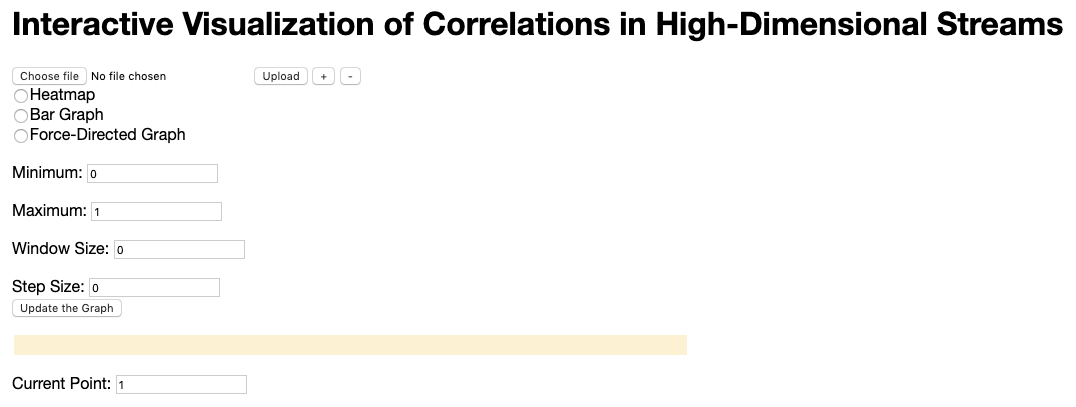
\includegraphics[width=15cm]{pictures/overview}
	\caption{Overview of the interface}
	\label{fig:overview}
\end{figure}

After pressing the \textbf{Upload} button, the data set will be stored at the back-end. The system calculates the correlations of each pair of attributes and the corresponding elements for performing the visualizations. If the calculation is finished, a confirm window will pop up to inform the maximal window size of the current data set to the user. The maximal window size is the whole size of the uploaded data. Also, the step size will be set to 1 and the window size will be set to the maximal window size after uploading the data set, see \autoref{fig:uploaded}.\\

\begin{figure}[h]
	\centering
	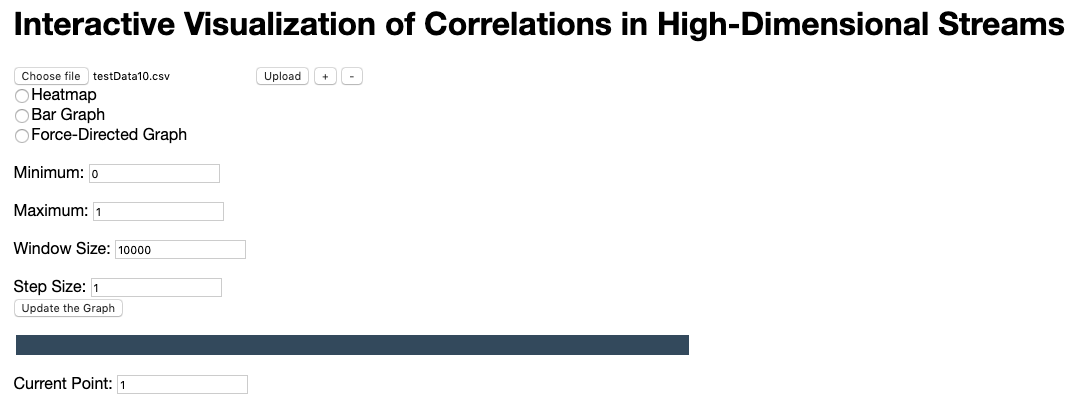
\includegraphics[width=15cm]{pictures/uploaded}
	\caption{After uploading a csv file}
	\label{fig:uploaded}
\end{figure}

Users are able to change the \textbf{minimum}, \textbf{maximum}, \textbf{window size}, \textbf{step size} and \textbf{current point}. After setting these values and pressing the \textbf{update} button, the visualization will be re-performed and the width of panel will be set to corresponding window size, seeing \autoref{fig:update}.\\

\begin{figure}[h]
	\centering
	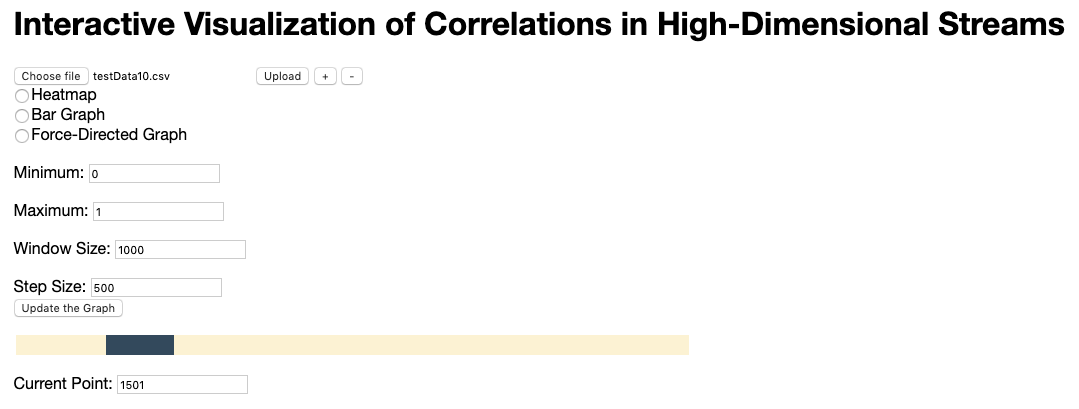
\includegraphics[width=15cm]{pictures/update}
	\caption{After pressing the "update" button}
	\label{fig:update}
\end{figure}

Our interface provides three visualization methods: Heatmap, Bar Graph and Force-Directed-Graph. After selecting the corresponding radio button, a visualization will be drawn on the web site. The \autoref{fig:choose} shows three visualizations based on the same data set we introduced in \autoref{sec:Visualization:mtcars}. \autoref{fig:chooseHM} is the Heatmap. Each box represents a pair of attributes and the color of the box represents the correlation value of this pair. \autoref{fig:chooseBar} is the Bar Graph, in which the height of each bar represents the correlation value of each pair of attributes. As 0 is not likely to be seen in case of many pairs of attributes, we paint the hole bar red and set the height to the maximal height. And \autoref{fig:chooseFDG} is the Force-Directed-Graph, in which the length of link between two nodes represents the correlation value of this pair of attributes. The shorter the linked distance is, the bigger is the correlation value. Users can also change the minimal and maximal correlation value they want to visualize, and slide the slider to see different time period of the current data set.

\begin{figure}[h]
	\centering
	\begin{subfigure}[b]{0.32\textwidth}
	\centering
	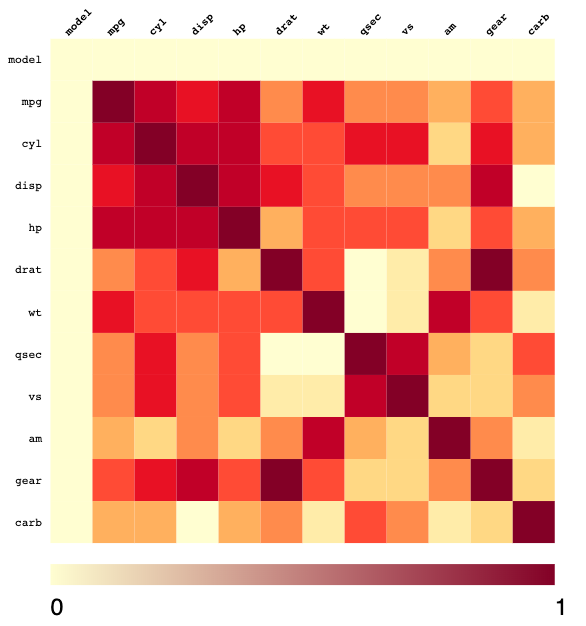
\includegraphics[width=\textwidth]{pictures/correlationMatrix}
	\caption{Select Heatmap as the visualization method}
		\label{fig:chooseHM}
\end{subfigure}
\hfill
\begin{subfigure}[b]{0.32\textwidth}
	\centering
	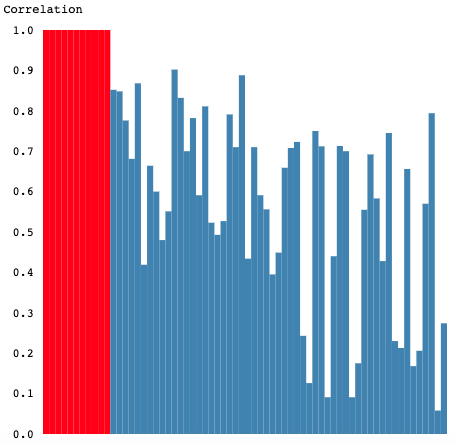
\includegraphics[width=\textwidth]{pictures/bg}
	\caption{Select Bar Graph as the visualization method}
		\label{fig:chooseBar}
\end{subfigure}
\hfill
\begin{subfigure}[b]{0.32\textwidth}
	\centering
	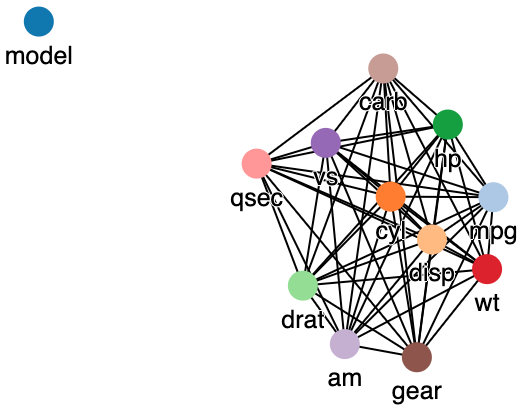
\includegraphics[width=\textwidth]{pictures/fdg}
	\caption{Select Force-Directed-Graph as the visualization method}
		\label{fig:chooseFDG}
\end{subfigure}
	\caption{Select different visualization methods}
	\label{fig:choose}
\end{figure}




%\chapter{Second Content Chapter}
%\label{ch:SecondContent}

%\dots

%\section{Second Section}
%\label{sec:SecondContent:SecondSection}

%\dots

%Add additional content chapters if required by adding new .tex files in the
%\code{sections/} directory and adding an appropriate 
%\code{\textbackslash input} statement in \code{thesis.tex}. 
%% ---------------------
%% | / Example content |
%% ---------------------

	%% LaTeX2e class for student theses
%% sections/evaluation.tex
%% 
%% Karlsruhe Institute of Technology
%% Institute for Program Structures and Data Organization
%% Chair for Software Design and Quality (SDQ)
%%
%% Dr.-Ing. Erik Burger
%% burger@kit.edu
%%
%% Version 1.3.3, 2018-04-17

\chapter{Evaluation Via User Studies}
\label{ch:Evaluation}

\section{Experimental Settings}
\label{sec:Evaluation:ExperimentalSettings}
In this thesis, we compare three different visualization methods, namely the so-called “Heatmap”, “Bar Graph” and “Force-Direct-Graph”. The participants are assessed with respect to different conditions, to which they will be assigned randomly. Participants are not aware of the condition they are assigned to: 
\begin{itemize}
	\item \textbf{Condition A}: Participants can only use the Heatmap and \autoref{fig:mockup_hm} is its mock-up
	\begin{figure}[htb]
		\centering
		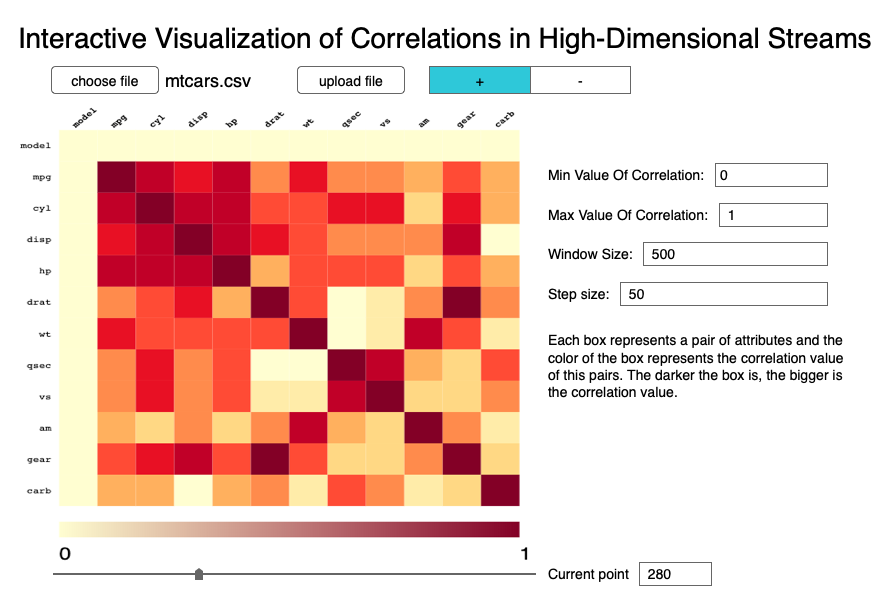
\includegraphics[width=15cm]{pictures/mockup_hm}
		\caption{Mock-up for Condition A}
		\label{fig:mockup_hm}
	\end{figure}

	\item \textbf{Condition B}: Participants can only use the Bar Graph and \autoref{fig:mockup_bg} is its mock-up
	\begin{figure}[htb]
		\centering
		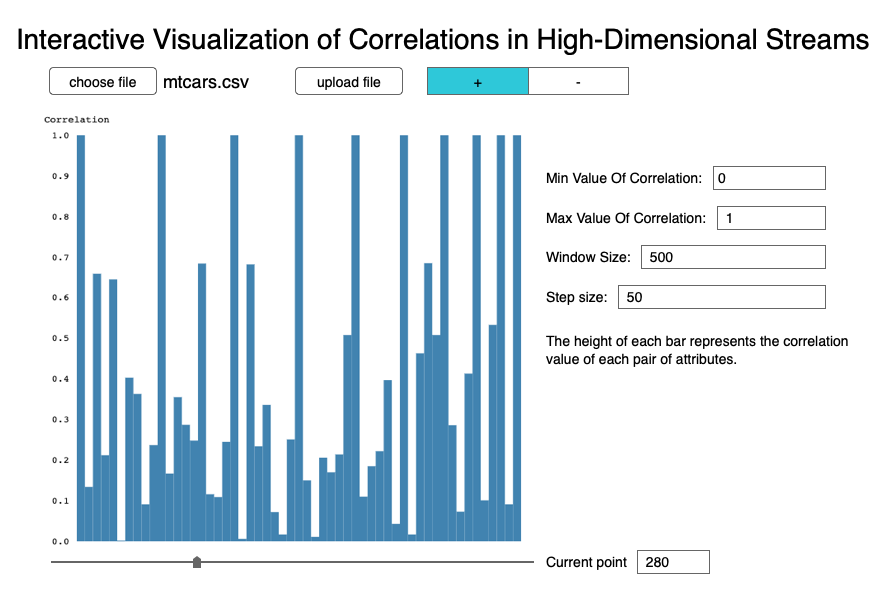
\includegraphics[width=15cm]{pictures/mockup_bg}
		\caption{Mock-up for Condition B}
		\label{fig:mockup_bg}
	\end{figure}
	
	\item \textbf{Condition C}: Participants can only use the Force-Directed-Graph and \autoref{fig:mockup_fdg} is its mock-up
	\begin{figure}[htb]
		\centering
		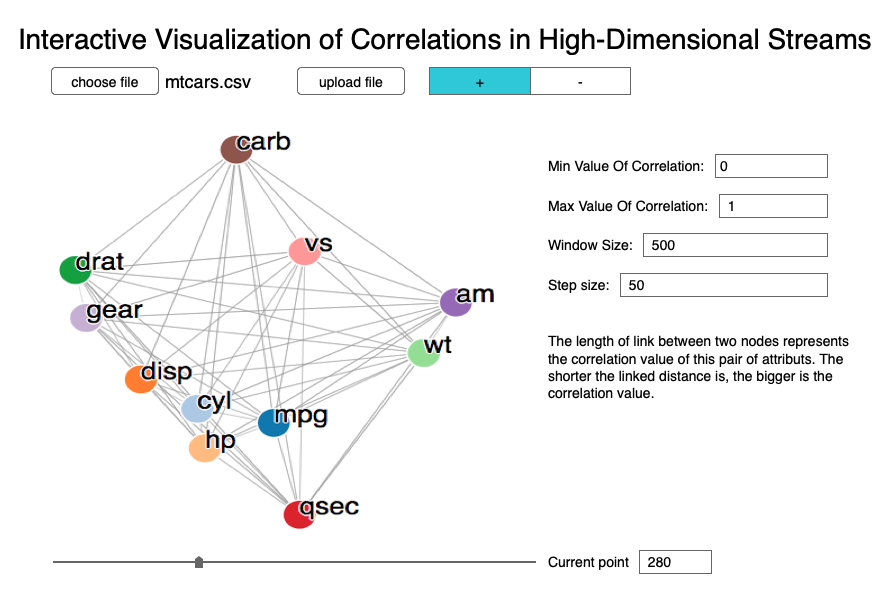
\includegraphics[width=15cm]{pictures/mockup_fdg}
		\caption{Mock-up for Condition C}
		\label{fig:mockup_fdg}
	\end{figure}
	
	\item \textbf{Condition D}: Participants can use any visualization method they want,which are mentioned in Condition A,B and C, and \autoref{fig:mockup} is its mock-up
		\begin{figure}[htb]
		\centering
		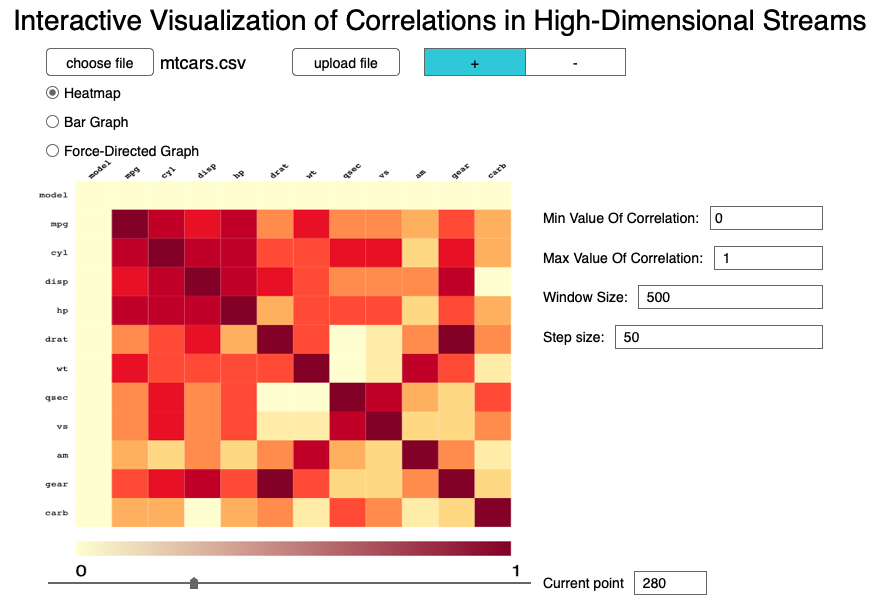
\includegraphics[width=15cm]{pictures/mockup_3}
		\caption{Mock-up for Condition D}
		\label{fig:mockup_3}
	\end{figure}
\end{itemize}

\subsection{Participants Profiles}
\label{sec:Evaluation:ExperimentalSettings:PP}
The participants we are looking for are adults who at least have the basic knowledge about browsing web page, typically 14 to 40 years old. We will sample a large share of our participants from the pool of students at KIT, so we may expect basic knowledge of computer science and data analysis.\\
Knowledge in data analysis and correlation analysis should not be required to use the prototype for the visualization of a data set. Still, we hypothesis that participants with prior exposure to data visualization will require less time to fulfill the tasks.\\

\subsection{Data Set}
\label{sec:Evaluation:ExperimentalSettings:DataSet}
The participant of user study are asked to use a data set taken at random from a pool of 3 data sets in total for completing the tasks. \textbf{Data Set 1 (DS1)} has 10 attributes within 2000 timestamps. \textbf{Data Set 2 (DS2)} has 20 attributes within 2000 timestamps. \textbf{Data Set 3 (DS3)} has 40 attributes within 2000 timestamps. These 3 data sets are actually the subsets of a real-world data set. For the evaluation, we make some modifications of this data set: reducing the number of attributes and selecting only 2000 instances of it. It is obvious that the difference between DS1, DS2 and DS3 are their level of difficulty according to their number of dimensions. In practice, this means that the same question will be harder to answer with DS3 than DS2 and DS1.\\

\subsection{Settings of interface}
The window size is set to 200 and the step size is set 50 for all three data sets, which cannot be changed by the participants.\\
During the user study, the participants are only able to change the minimum and maximum to filter the correlation values. Also, they can slide the sliding window or input "current point" to get the visualization graph of current timestamp.

\section{Questionnaire}
\label{sec:Evaluation:Questionnaire}
Before answering the questionnaire, all participants are asked to sign a Consent Form, shown in \autoref{cf}. The questionnaire is divided into 3 parts. In the first part of questionnaire \autoref{sec:Evaluation:Questionnaire}, the participants are asked to give some basic information. In the second part of questionnaire, the participants have to answer some questions using different visualization methods. \autoref{sec:Evaluation:Questionnaire:V} shows the question types and each question type will be asked three time in the user study. \autoref{sec:Evaluation:Questionnaire:F} is the last part of questionnaire, which introduces the feedback of using this interface. Participants under Condition A/B/C are asked to give feedback of the corresponding visualization methods they use, while participants under Condition D have to give feedback of each visualization method and the whole system.
\subsection{Basic Information}
\label{sec:Evaluation:Questionnaire:BI}
\begin{itemize}
	\item Field of study
	\item Number of semester
	\item Age:\\
	\begin{tabular}{| l | c | r |}
		\hline
		18-24 & 25-30 & More than 30 \\ \hline
	\end{tabular}
	\item Gender:\\
		\begin{tabular}{| l | c | r |}
		\hline
		M & F & Do not wish to answer \\ \hline
	\end{tabular}
	\item How familiar are you with the following concepts?
\begin{center}
	\begin{tabular}{ | l | l | l | l | l | l | l | l |}
		\hline
		                              & 1 (Unfamiliar) & 2 & 3 & 4 & 5 & 6 & 7 (Very Familiar) \\ \hline
		\textbf{Correlation analysis} &                &   &   &   &   &   &                   \\ \hline
		\textbf{Data analysis}        &                &   &   &   &   &   &                   \\ \hline
		\textbf{Data visualization}   &                &   &   &   &   &   &                   \\ \hline
	\end{tabular}
\end{center}
\end{itemize}

\subsection{Visualization}
\label{sec:Evaluation:Questionnaire:V}
\begin{itemize}
\item How many attributes are available in this data set?
\item How many pairs of attributes are available in this data set?
\item What is the correlation value between \textit{\textbf{\underline{Attribute A}}} and \textit{\textbf{\underline{Attribute B}}} at \textit{\textbf{\underline{Timestamp T}}}, or the probable range?
\item Which pair of attributes has the biggest correlation at \underline{\textbf{\textit{Timestamp T}}}?
\item Which pair of attributes has the smallest correlation at \underline{\textbf{\textit{Timestamp T}}}?
\item The following statement is true or false: “The correlation value between \underline{\textit{\textbf{Attribute A}}} and \underline{\textit{\textbf{Attribute B}}} remains the same at \underline{\textit{\textbf{Timestamp T1}}} and at \underline{\textit{\textbf{Timestamp T2}}}”?\\
	\begin{tabular}{| l | c |}
	\hline
	True & False \\ \hline
\end{tabular}
\item Which pair(s) of attributes has/have a correlation value that is not smaller than \underline{\textit{\textbf{X}}} at \underline{\textit{\textbf{Timestamp T}}}?
\item Which pair(s) of attributes has/have a correlation value that is not bigger than \underline{\textit{\textbf{X}}} at \underline{\textit{\textbf{Timestamp T}}}?
\end{itemize}

\subsection{Feedback}
\label{sec:Evaluation:Questionnaire:F}
\subsubsection{Participants Under Condition A/B/C}
Participants under Condition A, B and C are asked to give feedback based on following questions:
\begin{itemize}
	\item Please write down the visualization method you have used and rate for it.
	\begin{center}
		\begin{tabular}{ | l | l | l | l | l | l | l | l | }
			\hline
			                     & 1 (Strongly Disagree) & 2 & 3 & 4 & 5 & 6 & 7 (Strongly Agree) \\ \hline
			\textbf{Intuitive}   &                       &   &   &   &   &   &                    \\ \hline
			\textbf{Convenient}  &                       &   &   &   &   &   &                    \\ \hline
			\textbf{Interactive} &                       &   &   &   &   &   &                    \\ \hline
			\textbf{Useful}      &                       &   &   &   &   &   &                    \\ \hline
			\textbf{Complicated} &                       &   &   &   &   &   &                    \\ \hline
			\textbf{Efficient}   &                       &   &   &   &   &   &                    \\ \hline
			\textbf{Effective}   &                       &   &   &   &   &   &                    \\ \hline
		\end{tabular}
	\end{center}
\item In your opinion, what are the strengths of this visualization system?
\item In your opinion, what are the weaknesses of this visualization system?
\item Do you have any suggestions for improving this visualization system?
\end{itemize}

\subsubsection{Participants Under Condition D}
Participants under Condition D, who are able to use either of 3 visualization methods, are asked to give feedback to the whole system, which is also quite similar to the one for participants under Condition A, B or C. In addition, they need to give ratings for each visualization method.
\begin{itemize}
	\item As you are able to use all visualization methods during the research, which one of the method, in your opinion, is the most helpful method to fulfill the task?
	\item And which of the method did you use the most?
	\item Please rate for \textit{Heat map}:
		\begin{center}
		\begin{tabular}{ | l | l | l | l | l | l | l | l | }
			\hline
			& 1 (Strongly Disagree) & 2 & 3 & 4 & 5 & 6 & 7 (Strongly Agree) \\ \hline
			\textbf{Intuitive}   &                       &   &   &   &   &   &                    \\ \hline
			\textbf{Convenient}  &                       &   &   &   &   &   &                    \\ \hline
			\textbf{Interactive} &                       &   &   &   &   &   &                    \\ \hline
			\textbf{Useful}      &                       &   &   &   &   &   &                    \\ \hline
			\textbf{Complicated} &                       &   &   &   &   &   &                    \\ \hline
			\textbf{Efficient}   &                       &   &   &   &   &   &                    \\ \hline
			\textbf{Effective}   &                       &   &   &   &   &   &                    \\ \hline
		\end{tabular}
	\end{center}
		\item Please rate for \textit{Bar Graph}:
	\begin{center}
		\begin{tabular}{ | l | l | l | l | l | l | l | l | }
			\hline
			& 1 (Strongly Disagree) & 2 & 3 & 4 & 5 & 6 & 7 (Strongly Agree) \\ \hline
			\textbf{Intuitive}   &                       &   &   &   &   &   &                    \\ \hline
			\textbf{Convenient}  &                       &   &   &   &   &   &                    \\ \hline
			\textbf{Interactive} &                       &   &   &   &   &   &                    \\ \hline
			\textbf{Useful}      &                       &   &   &   &   &   &                    \\ \hline
			\textbf{Complicated} &                       &   &   &   &   &   &                    \\ \hline
			\textbf{Efficient}   &                       &   &   &   &   &   &                    \\ \hline
			\textbf{Effective}   &                       &   &   &   &   &   &                    \\ \hline
		\end{tabular}
	\end{center}
		\item Please rate for \textit{Force-Directed Graph}:
	\begin{center}
		\begin{tabular}{ | l | l | l | l | l | l | l | l | }
			\hline
			& 1 (Strongly Disagree) & 2 & 3 & 4 & 5 & 6 & 7 (Strongly Agree) \\ \hline
			\textbf{Intuitive}   &                       &   &   &   &   &   &                    \\ \hline
			\textbf{Convenient}  &                       &   &   &   &   &   &                    \\ \hline
			\textbf{Interactive} &                       &   &   &   &   &   &                    \\ \hline
			\textbf{Useful}      &                       &   &   &   &   &   &                    \\ \hline
			\textbf{Complicated} &                       &   &   &   &   &   &                    \\ \hline
			\textbf{Efficient}   &                       &   &   &   &   &   &                    \\ \hline
			\textbf{Effective}   &                       &   &   &   &   &   &                    \\ \hline
		\end{tabular}
	\end{center}
		\item Please rate for \textit{whole system}:
	\begin{center}
		\begin{tabular}{ | l | l | l | l | l | l | l | l | }
			\hline
			& 1 (Strongly Disagree) & 2 & 3 & 4 & 5 & 6 & 7 (Strongly Agree) \\ \hline
			\textbf{Intuitive}   &                       &   &   &   &   &   &                    \\ \hline
			\textbf{Convenient}  &                       &   &   &   &   &   &                    \\ \hline
			\textbf{Interactive} &                       &   &   &   &   &   &                    \\ \hline
			\textbf{Useful}      &                       &   &   &   &   &   &                    \\ \hline
			\textbf{Complicated} &                       &   &   &   &   &   &                    \\ \hline
			\textbf{Efficient}   &                       &   &   &   &   &   &                    \\ \hline
			\textbf{Effective}   &                       &   &   &   &   &   &                    \\ \hline
		\end{tabular}
	\end{center}
	\item In your opinion, what are the strengths of this visualization system?
	\item In your opinion, what are the weaknesses of this visualization system?
	\item Do you have any suggestions for improving this visualization system?
\end{itemize}

\section{Script For Conducting The Experiment}
\label{sec:Evaluation:Script}
\textit{\textbf{The following information will be given to the participants, orally:}}\\
Thank you for participating to this experiment. My name is Yimin Zhang. I am doing my Bachelor thesis in the Institute for Program Structures and Data Organization (IPD Böhm).\\
The goal of the experiment is to evaluate an interface that I have developed for my thesis. First of all, please read and sign the consent form. If you have any problems during the study, please be free to talk to me.\\
\textbf{\textit{(After signing)}}\\
Please fill in the blanks of the website about the basic information, which is the first part of the questionnaire: Section 1.\\
\textbf{\textit{(After Part 1)}}\\
Your task from now on is to upload the data set and to answer the questions in Part 2. You are free to use all the elements on the web page to ease the task. Please cross a question off, if you cannot answer the question. The time you need to answer for each question will also be recorded.\\
\textbf{\textit{(After Part 2)}}\\
The last task for you is to provide your personal feedback for this interface. This is the third part of the questionnaire.\\
\textbf{\textit{(After Part 3)}}\\
Thank you for participating in my study. If you are interested in my thesis or may have further questions, please be free to contact me using the contact information in the consent form. I wish you a nice day.\\

\section{Result}
\label{sec:Evaluation:Result}
We invited 22 students studying various fields at KIT to participate the user study. They are all studying 6 or higher semester and below 30 years old, 12 female students and 10 male students. \autoref{fig:statics1} shows the statics of basic information of these participants. The most unfamiliar concept for them is the data visualization, which reaches the average of 2.1. They are more familiar with correlation and data analysis, both with the average of 3.1.
\begin{figure}[h]
	\centering
	\begin{subfigure}[b]{0.48\textwidth}
		\centering
		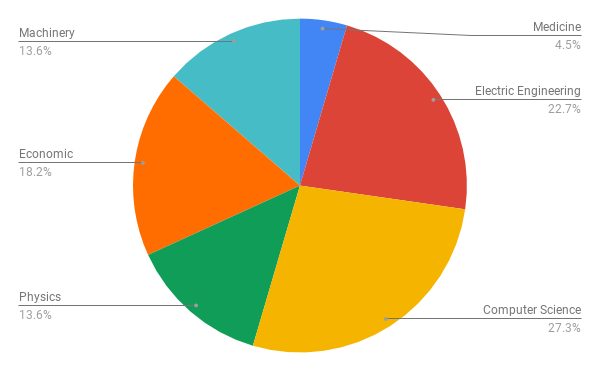
\includegraphics[width=\textwidth]{pictures/q11}
		\caption{Field of study}
	\end{subfigure}
	\hfill
	\begin{subfigure}[b]{0.48\textwidth}
		\centering
		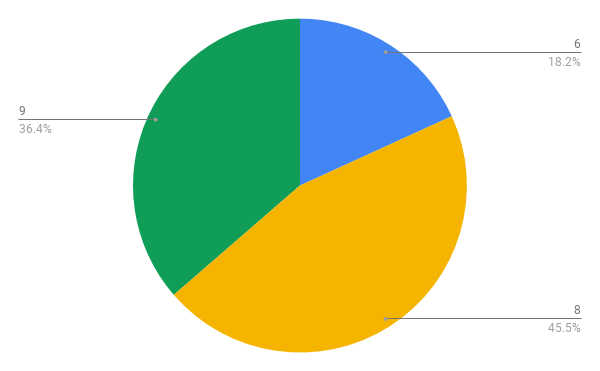
\includegraphics[width=\textwidth]{pictures/q12}
		\caption{Number of semester}
	\end{subfigure}
	\hfill
	\begin{subfigure}[b]{0.48\textwidth}
		\centering
		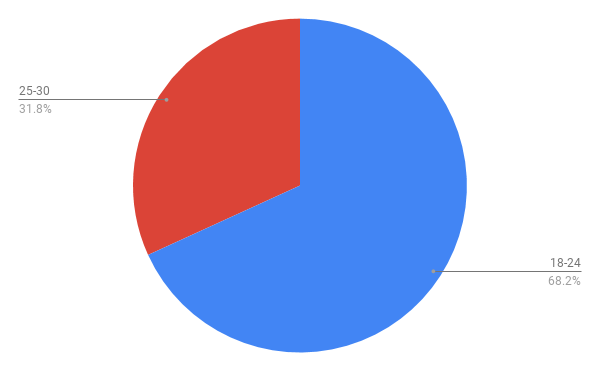
\includegraphics[width=\textwidth]{pictures/q13}
		\caption{Age}
	\end{subfigure}
	\begin{subfigure}[b]{0.48\textwidth}
	\centering
	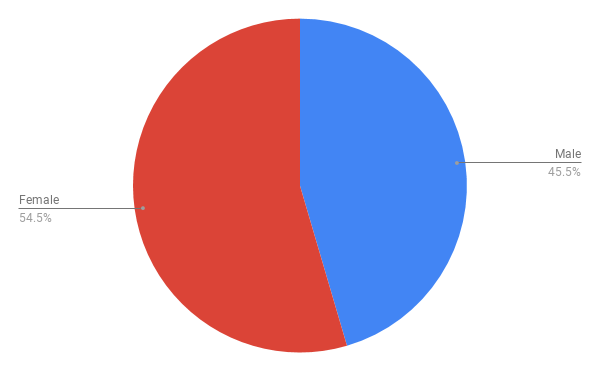
\includegraphics[width=\textwidth]{pictures/q14}
	\caption{Gender}
\end{subfigure}
	\begin{subfigure}[b]{\textwidth}
	\centering
	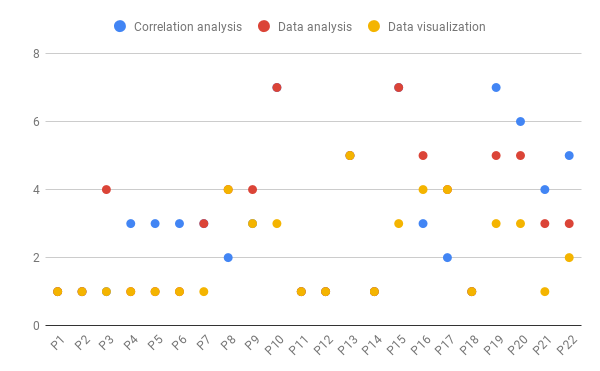
\includegraphics[width=\textwidth]{pictures/q15}
	\caption{How familiar are you with the following concepts?}
\end{subfigure}
	\caption{Statics of basic information}
	\label{fig:statics1}
\end{figure}

\subsection{Statics about the visualization part}
\begin{figure}[h]
	\centering
	\begin{subfigure}[b]{0.48\textwidth}
		\centering
		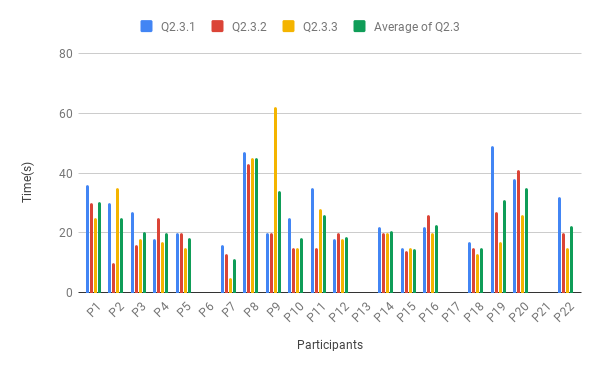
\includegraphics[width=\textwidth]{pictures/q23}
		\caption{Time for Question Q2.3}
	\end{subfigure}
	\hfill
	\begin{subfigure}[b]{0.48\textwidth}
		\centering
		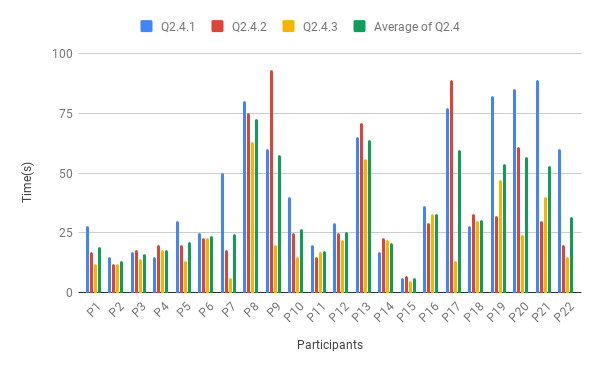
\includegraphics[width=\textwidth]{pictures/q24}
		\caption{Time for Question Q2.4}
	\end{subfigure}
	\hfill
	\begin{subfigure}[b]{0.48\textwidth}
		\centering
		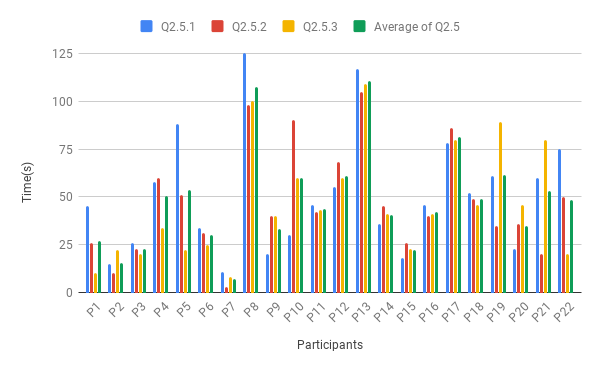
\includegraphics[width=\textwidth]{pictures/q25}
		\caption{Time for Question Q2.5}
	\end{subfigure}
	\begin{subfigure}[b]{0.48\textwidth}
		\centering
		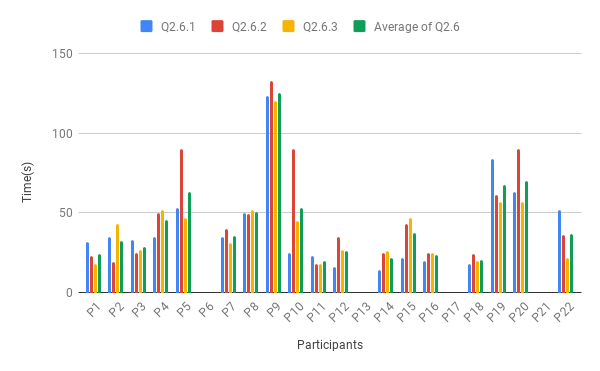
\includegraphics[width=\textwidth]{pictures/q26}
		\caption{Time for Question Q2.6}
	\end{subfigure}
	\begin{subfigure}[b]{0.48\textwidth}
		\centering
		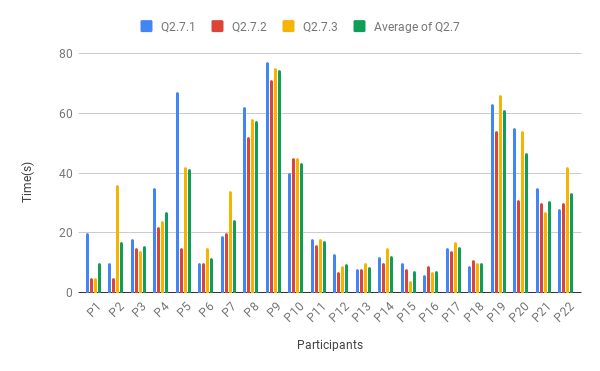
\includegraphics[width=\textwidth]{pictures/q27}
		\caption{Time for Question Q2.7}
	\end{subfigure}
	\begin{subfigure}[b]{0.48\textwidth}
	\centering
	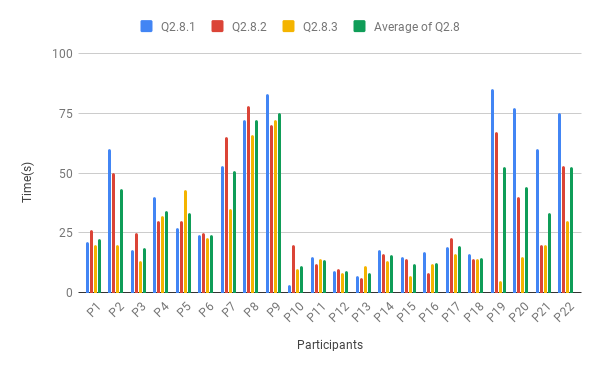
\includegraphics[width=\textwidth]{pictures/q28}
	\caption{Time for Question Q2.8}
\end{subfigure}
	\caption{Time of each participant finishing questions}
	\label{fig:statics2}
\end{figure}

\begin{figure}[h]
	\centering
	\begin{subfigure}[b]{0.48\textwidth}
		\centering
		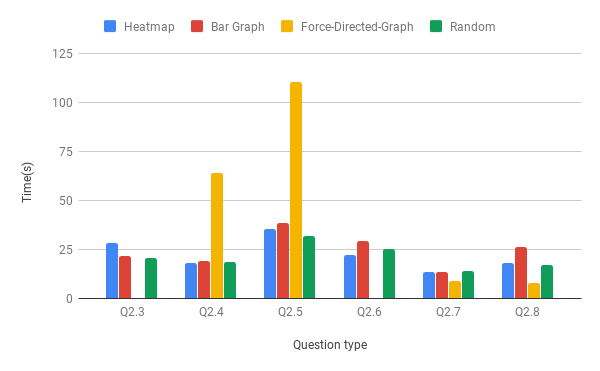
\includegraphics[width=\textwidth]{pictures/Time1}
		\caption{Use Data Set 1}
	\end{subfigure}
	\hfill
	\begin{subfigure}[b]{0.48\textwidth}
		\centering
		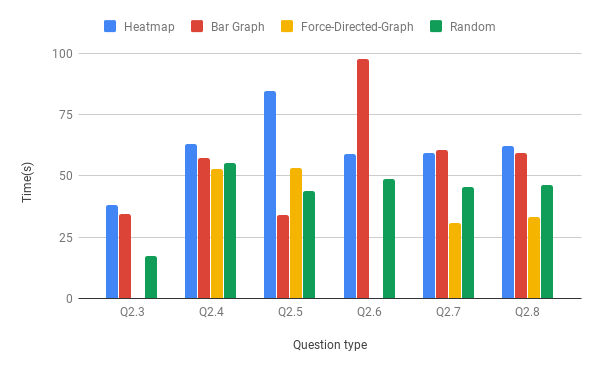
\includegraphics[width=\textwidth]{pictures/Time2}
		\caption{Use Data Set 2}
	\end{subfigure}
	\hfill
	\begin{subfigure}[b]{0.48\textwidth}
		\centering
		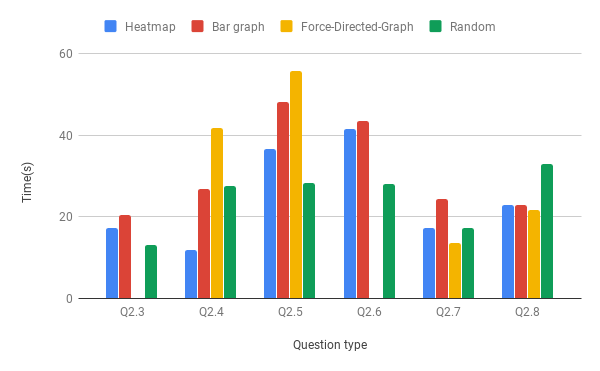
\includegraphics[width=\textwidth]{pictures/Time3}
		\caption{Use Data Set 3}
	\end{subfigure}
	\caption{Average time of participants finishing each question type using different data sets}
	\label{fig:averageDS}
\end{figure}

\begin{figure}[h]
	\centering
	\begin{subfigure}[b]{0.48\textwidth}
		\centering
		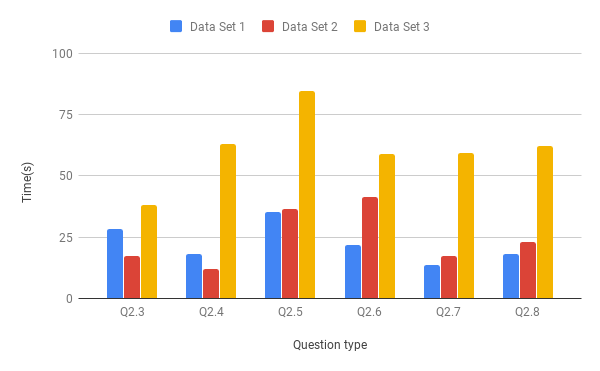
\includegraphics[width=\textwidth]{pictures/TimeH}
		\caption{Use Heatmap as visualization method}
	\end{subfigure}
	\hfill
	\begin{subfigure}[b]{0.48\textwidth}
		\centering
		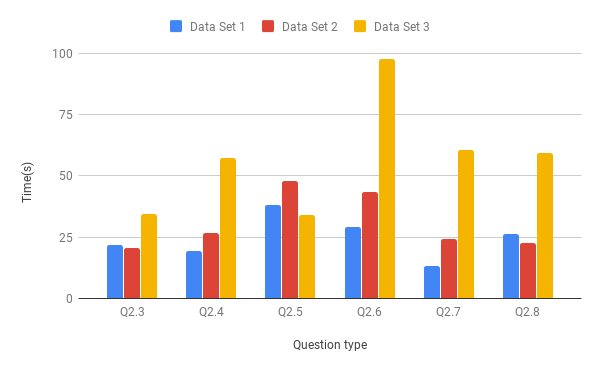
\includegraphics[width=\textwidth]{pictures/TimeB}
		\caption{Use Bar Graph as visualization method}
	\end{subfigure}
	\hfill
	\begin{subfigure}[b]{0.48\textwidth}
		\centering
		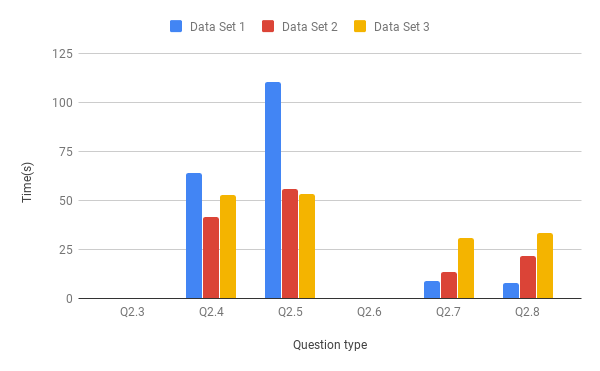
\includegraphics[width=\textwidth]{pictures/TimeF}
		\caption{Use Force-Directed-Graph as visualization method}
	\end{subfigure}
	\begin{subfigure}[b]{0.48\textwidth}
	\centering
	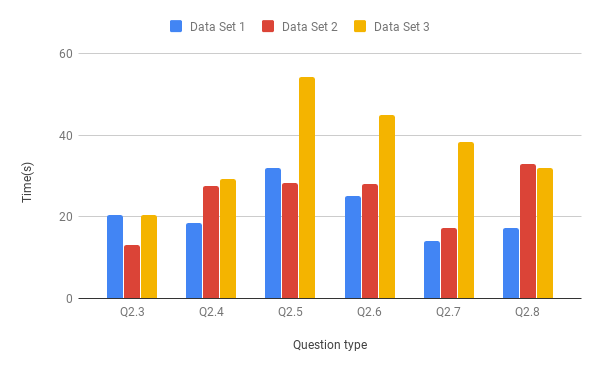
\includegraphics[width=\textwidth]{pictures/TimeD}
	\caption{Use random visualization method}
\end{subfigure}
	\caption{Average time of participants finishing each question type using different visualization methods}
	\label{fig:averageV}
\end{figure}

\begin{figure}[h]
	\centering
	\begin{subfigure}[b]{0.48\textwidth}
		\centering
		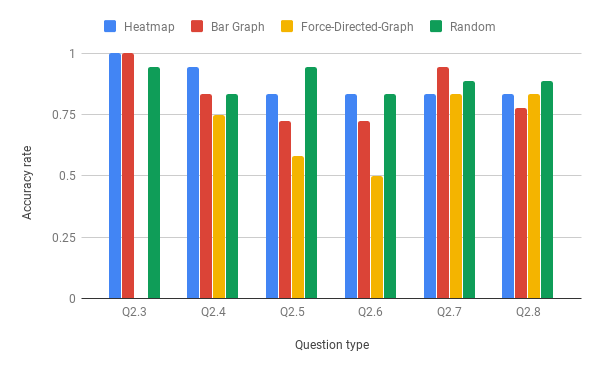
\includegraphics[width=\textwidth]{pictures/accuracy}
		\caption{Accuracy rate of each question type using different visualization methods}
		\label{fig:accuracyV}
	\end{subfigure}
	\hfill
	\begin{subfigure}[b]{0.48\textwidth}
		\centering
		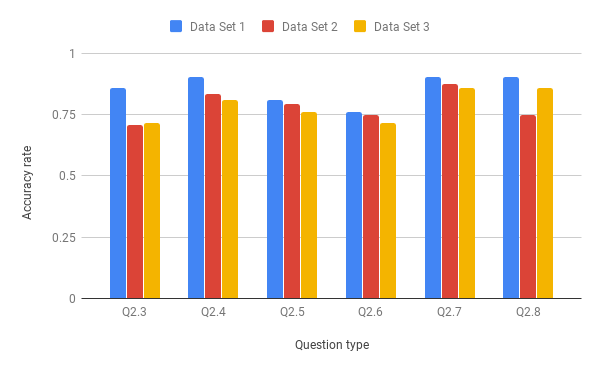
\includegraphics[width=\textwidth]{pictures/accuracyDS}
		\caption{Accuracy rate of each question type using different data sets}
		\label{fig:accuracyDS}
	\end{subfigure}
	\caption{Accuracy rate of each question type}
	\label{fig:accuracy}
\end{figure}

Questions about the number of attributes and pairs of correlations are answered correctly by all the participants. The time they used to answer the other questions are recorded and analyzed in \autoref{fig:statics2}. \autoref{fig:averageDS} shows the statics about the average time of participants using different data sets to finish each question type. It is obvious that both the average time of using Heatmap and Bar Graph is close whatever data set the participants use. When using Force-Directed-Graph, the participants need more time. The time for participants who can use all three visualization methods is also similar to the time using Heatmap/Bar Graph.\\
\autoref{fig:averageV} shows the average time of participants using different visualization methods to finish each question type. We can conclude from the figure that the time for the participants to finish the questions is mostly in direct proportion to the size of the data set, which is also related to the number of pairs for correlations.\\
\autoref{fig:accuracyV} shows the accuracy rate of each question type using different visulization methods. All the accuracy rates are over 50\%. When being able to use Heatmap or 3 visualization methods at random, the accuracy rate even climbs to 75\%. However, for questions asking about the precision, like \textbf{Q2.3}: What is the correlation value between \textit{\textbf{\underline{Attribute A}}} and \textit{\textbf{\underline{Attribute B}}} at \textit{\textbf{\underline{Timestamp T}}}, or the probable range?, the participants are not able to give out their answers by using Force-Directed-Graph. We can infer that Force-Directed-Graph is more suitable to analyze the relationship between attributes than to have a precise value. The accuracy rate of each question type using different data sets is shown in \autoref{fig:accuracyDS}. We can see that using the smallest data set: Data Set 1, always results in the highest accuracy rate.

\subsection{Feedback}
From the survey, we have found out that the Heatmap and Bar Graph are the most often-used visualization methods. We can infer that although they can use three visualization methods in random, they are not quite likely to use Force-Directed-Graph to answer the questions. The ratings for each visualization method and the interface is displayed on the following table:
	\begin{center}
	\begin{tabular}{ | l | l | l | l | l | }
		\hline
		                     & Heatmap & Bar Graph & Force-Directed-Graph & Interface \\ \hline
		\textbf{Intuitive}   & 5.83    & 6.17      & 3.5                  & 6         \\ \hline
		\textbf{Convenient}  & 5.33    & 5.67      & 3.17                 & 5.83      \\ \hline
		\textbf{Interactive} & 5.83    & 5.67      & 4.17                 & 6.16      \\ \hline
		\textbf{Useful}      & 6       & 5.67      & 3.33                 & 5.83      \\ \hline
		\textbf{Complicated} & 2.67    & 3         & 4                    & 3.17      \\ \hline
		\textbf{Efficient}   & 5.33    & 5         & 3.33                 & 5.83      \\ \hline
		\textbf{Effective}   & 5.5     & 5.67      & 3.67                 & 5.67      \\ \hline
	\end{tabular}
\end{center}
From the table, we can see that the Force-Directed-Graph is the most complicated visualization methods for participants. Most participants found Heatmap and Bar Graph very intuitive in data visualization. In the feedback, intuition is one of the strength of this visualization system. In addition, this system meets many demands for data processing. As we have three visualization methods, each method can be used for different use to ease the correlation analysis. It is also interesting to see the change of graphs by sliding the sliding window.\\
The maximal value is very easy to find out by the interface, but when it comes to a relative small correlation value, it is quite hard for participants. Although different color of blocks represents different value in Heatmap, the blocks looks the same when the difference of two values is small, e.g. 0.005. Also, when the number of correlations is big, it's labored to see through the bars to find the change of one pair of attributes. Thanks to the filtering of minimal and maximal values of correlation values, the participants can save some time and strength to analyze the data.\\
The participants are glad to see more visualization methods and to use more functions of this interface. It is suggested that the interface is not only used for correlation analysis, but also for data analysis and have functions like mean, variance and median. Also, it could be helpful to output the exact correlation value of one pair by inputting the names of attributes. For Bar Graph, sort functions to re-arrange the order is quite useful to find certain pairs. As the Force-Directed-Graph shows the relationships of attributes, it is interesting when one node is pointed, only the related links will be shown. Also, only showing small sub-groups of the attributes can be helpful.
	%% LaTeX2e class for student theses
%% sections/conclusion.tex
%% 
%% Karlsruhe Institute of Technology
%% Institute for Program Structures and Data Organization
%% Chair for Software Design and Quality (SDQ)
%%
%% Dr.-Ing. Erik Burger
%% burger@kit.edu
%%
%% Version 1.3.3, 2018-04-17

\chapter{Conclusion}
\label{ch:Conclusion}
Correlation analysis is one of the fundamental task of Data Mining. It aims at discovering and summarizing the relationship between the attributes of a data set. Knowing the relationship between a set of variables, one can infer useful knowledge about external, a priori unknown outcomes. The evolving nature of streams and the high-dimensionality are two main challenges of analyzing high-dimensional data streams.\\
The goal of this thesis is the development of an interface for visualization of correlation in high-dimensional streams. We compare three different visualization methods through this interface: Heatmap, Bar Graph and Force-Directed-Graph. Our interactive interface reflects a tendency of the data correlation by visualization throughout the time. Users are able to choose a certain period of time to perform the correlation analysis and visualization. It is easy and quick for users to find pairs of attributes with strong correlations and also to see the evolution of data set during the time. This interface makes it possible to have a first glance at the data and provides some basic information before starting detailed analysis.\\
With the help of feedback from controlled user study, more useful functions can be added to our interface in order to ease the correlation analysis. Also, this interface can have more visualization methods than Heatmap, Bar Graph and Force-Directed-Graph and the current existing visualization methods can still be improved. In our thesis, we only focus on pairwise relationships and the correlations between more than two variables may remain to be discovered in the future work.\\



%% -------------------
%% | Example content |
%% -------------------

%This is the SDQ thesis template.
%For more information on the formatting of theses at SDQ, please refer to
%\url{https://sdqweb.ipd.kit.edu/wiki/Ausarbeitungshinweise} or to your advisor.

%\section{Example: Citation}
%\label{sec:Introduction:Citation}
%A citation: \cite{becker2008a} For referencing, see \autoref{sec:Introduction:Figures}

%\section{Example: Figures}
%\label{sec:Introduction:Figures}
%\begin{figure}[h]
%	\centering
%	
\includegraphics[width=4cm]{logos/sdqlogo}
%	\caption{SDQ logo}
%	\label{fig:sdqlogo}
%\end{figure}

%A reference: The SDQ logo is displayed in \autoref{fig:sdqlogo}. (Use \code{\textbackslash autoref\{\}} for easy referencing.) 

%\section{Example: Tables}
%\label{sec:Introduction:Tables}
%\begin{table}[h]
%	\centering
%	\begin{tabular}{r l}
	%	\toprule
	%	abc & def\\
	%	ghi & jkl\\
	%	\midrule
	%	123 & 456\\
	%	789 & 0AB\\
	%	\bottomrule
%	\end{tabular}
%	\caption{A table}
%	\label{tab:atable}
%\end{table}

%\section{Example: Todo-Note}
%Meaningless text.

%\section{Example: Formula}
%One of the nice things about the Linux Libertine font is that it comes with a math mode package.
%\begin{displaymath}
%f(x)=\Omega(g(x))\ (x\rightarrow\infty)\;\Leftrightarrow\;
%\limsup_{x \to \infty} \left|\frac{f(x)}{g(x)}\right|> 0
%\end{displaymath}

%% --------------------
%% | /Example content |
%% --------------------

%% -------------------
%% | Example content |
%% -------------------
%The content chapters of your thesis should of course be renamed. How many chapters you need to write depends on your thesis and cannot be said in general.

%Check out the examples theses in the SDQWiki:

%\url{https://sdqweb.ipd.kit.edu/wiki/Abschlussarbeit/Studienarbeit}

%Of course, you can split this .tex file into several files if you prefer. 









	
	%% --------------------
	%% |   Bibliography   |
	%% --------------------
	
	%% Add entry to the table of contents for the bibliography
    \bibliographystyle{acm}
    \bibliography{thesis}
	%\printbibliography[heading=bibintoc]
	
	%% ----------------
	%% |   Appendix   |
	%% ----------------
	%\appendix
	%% LaTeX2e class for student theses
%% sections/apendix.tex
%% 
%% Karlsruhe Institute of Technology
%% Institute for Program Structures and Data Organization
%% Chair for Software Design and Quality (SDQ)
%%
%% Dr.-Ing. Erik Burger
%% burger@kit.edu
%%
%% Version 1.3.3, 2018-04-17

%\iflanguage{english}
\chapter{Appendix}    % english style
%{\chapter{Anhang}}      % german style
\label{chap:appendix}
\section{Consent Form}
\label{cf}
	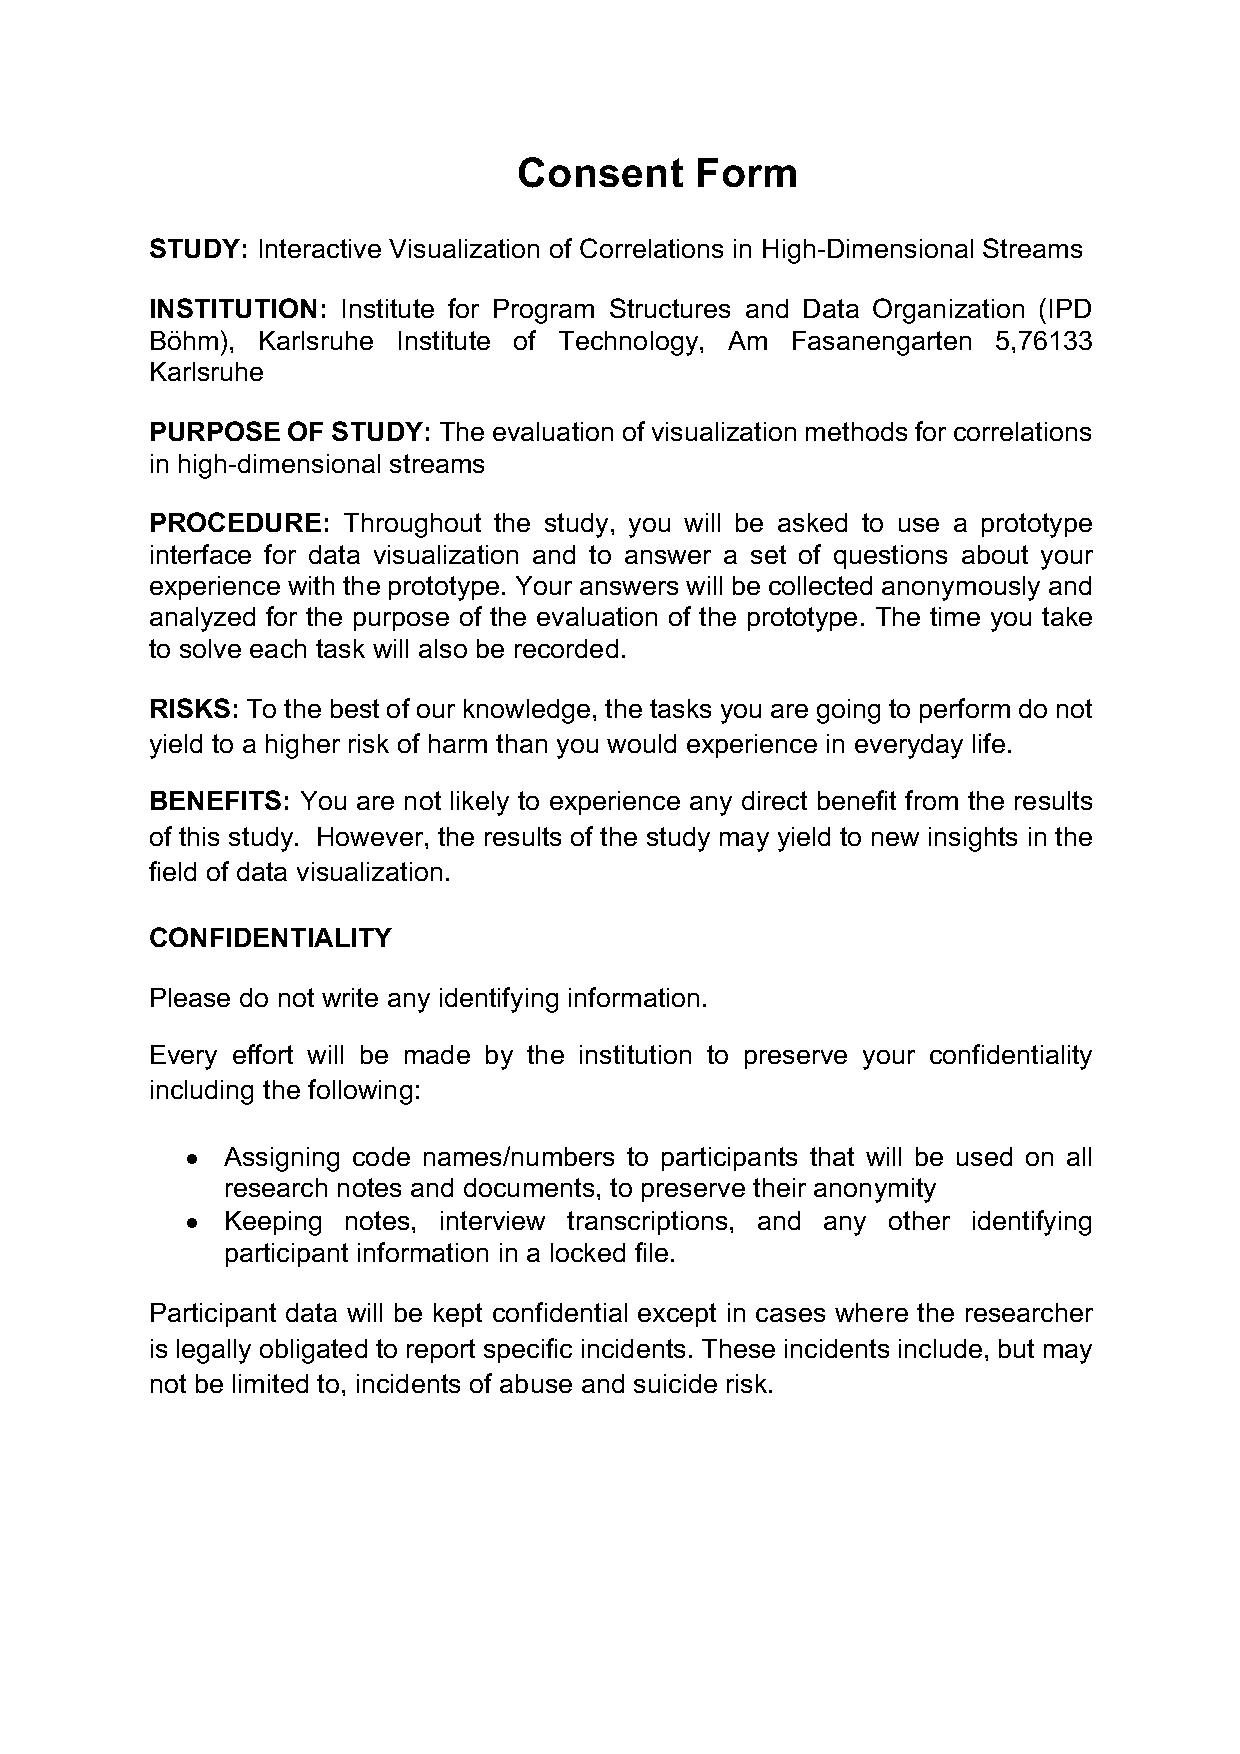
\includegraphics[scale=0.8]{us/ConsentForm1.pdf}
	\newpage
	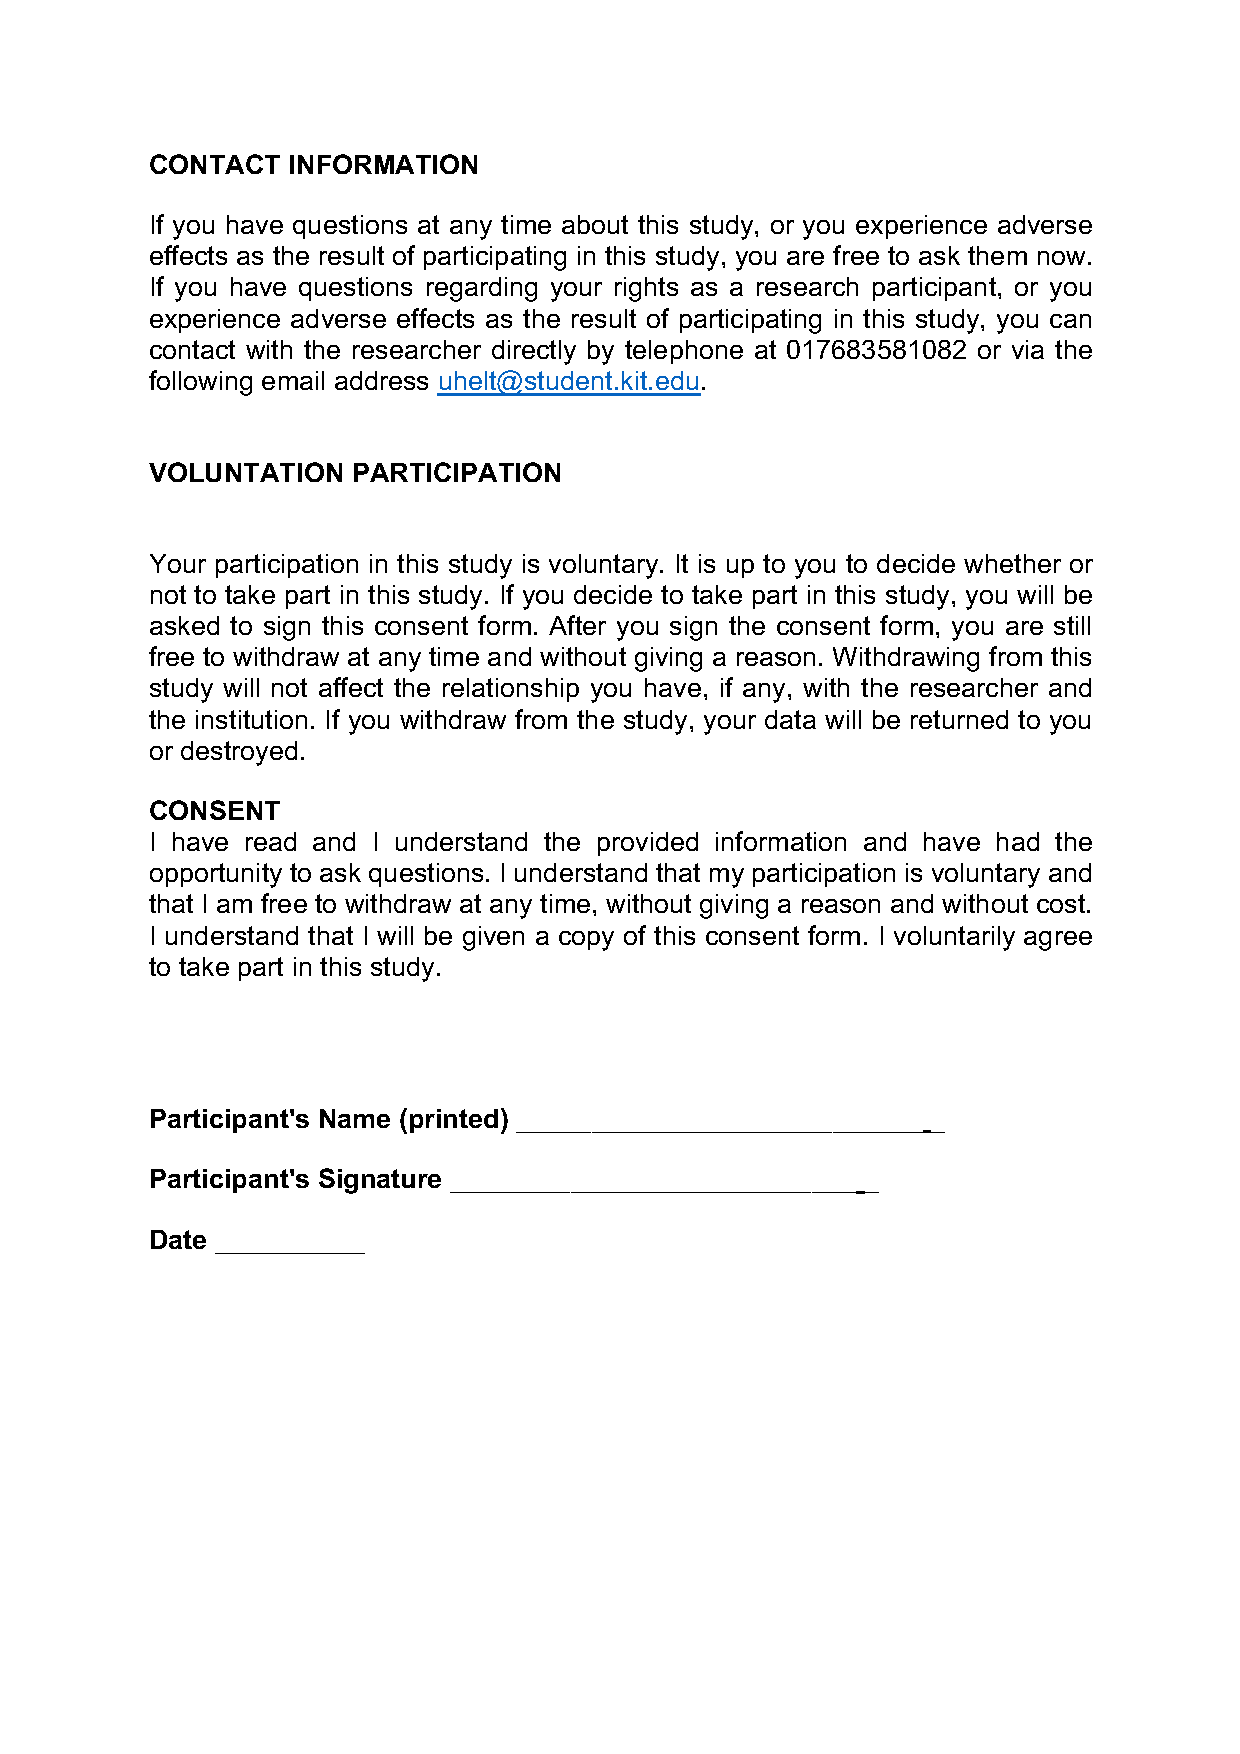
\includegraphics[scale=0.8]{us/ConsentForm2.pdf}
	
\section{Questionnaire}
\subsection{Questionnaire For Participants under Condition A/B/C}
\subsubsection{Participants using Data Set 1}
	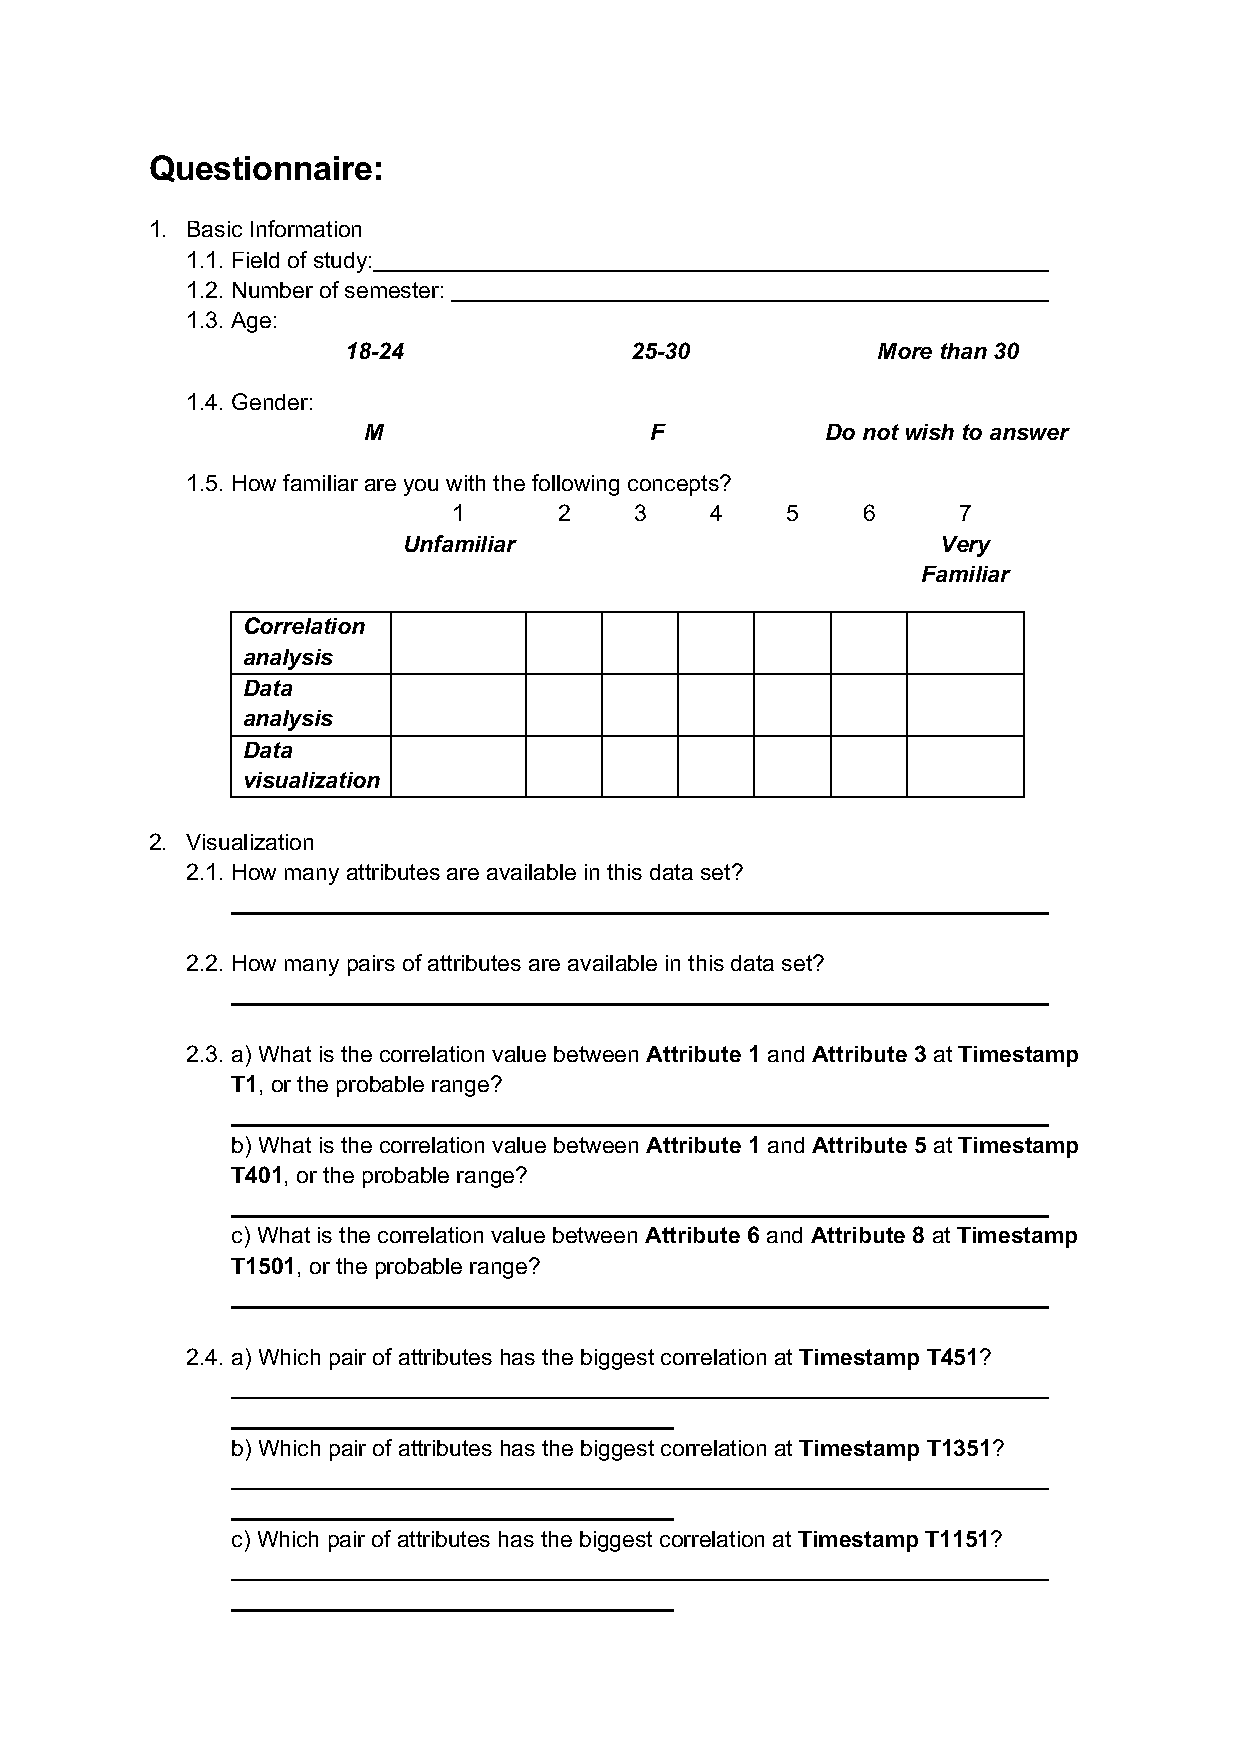
\includegraphics[scale=0.8]{us/q101.pdf}
	\newpage
	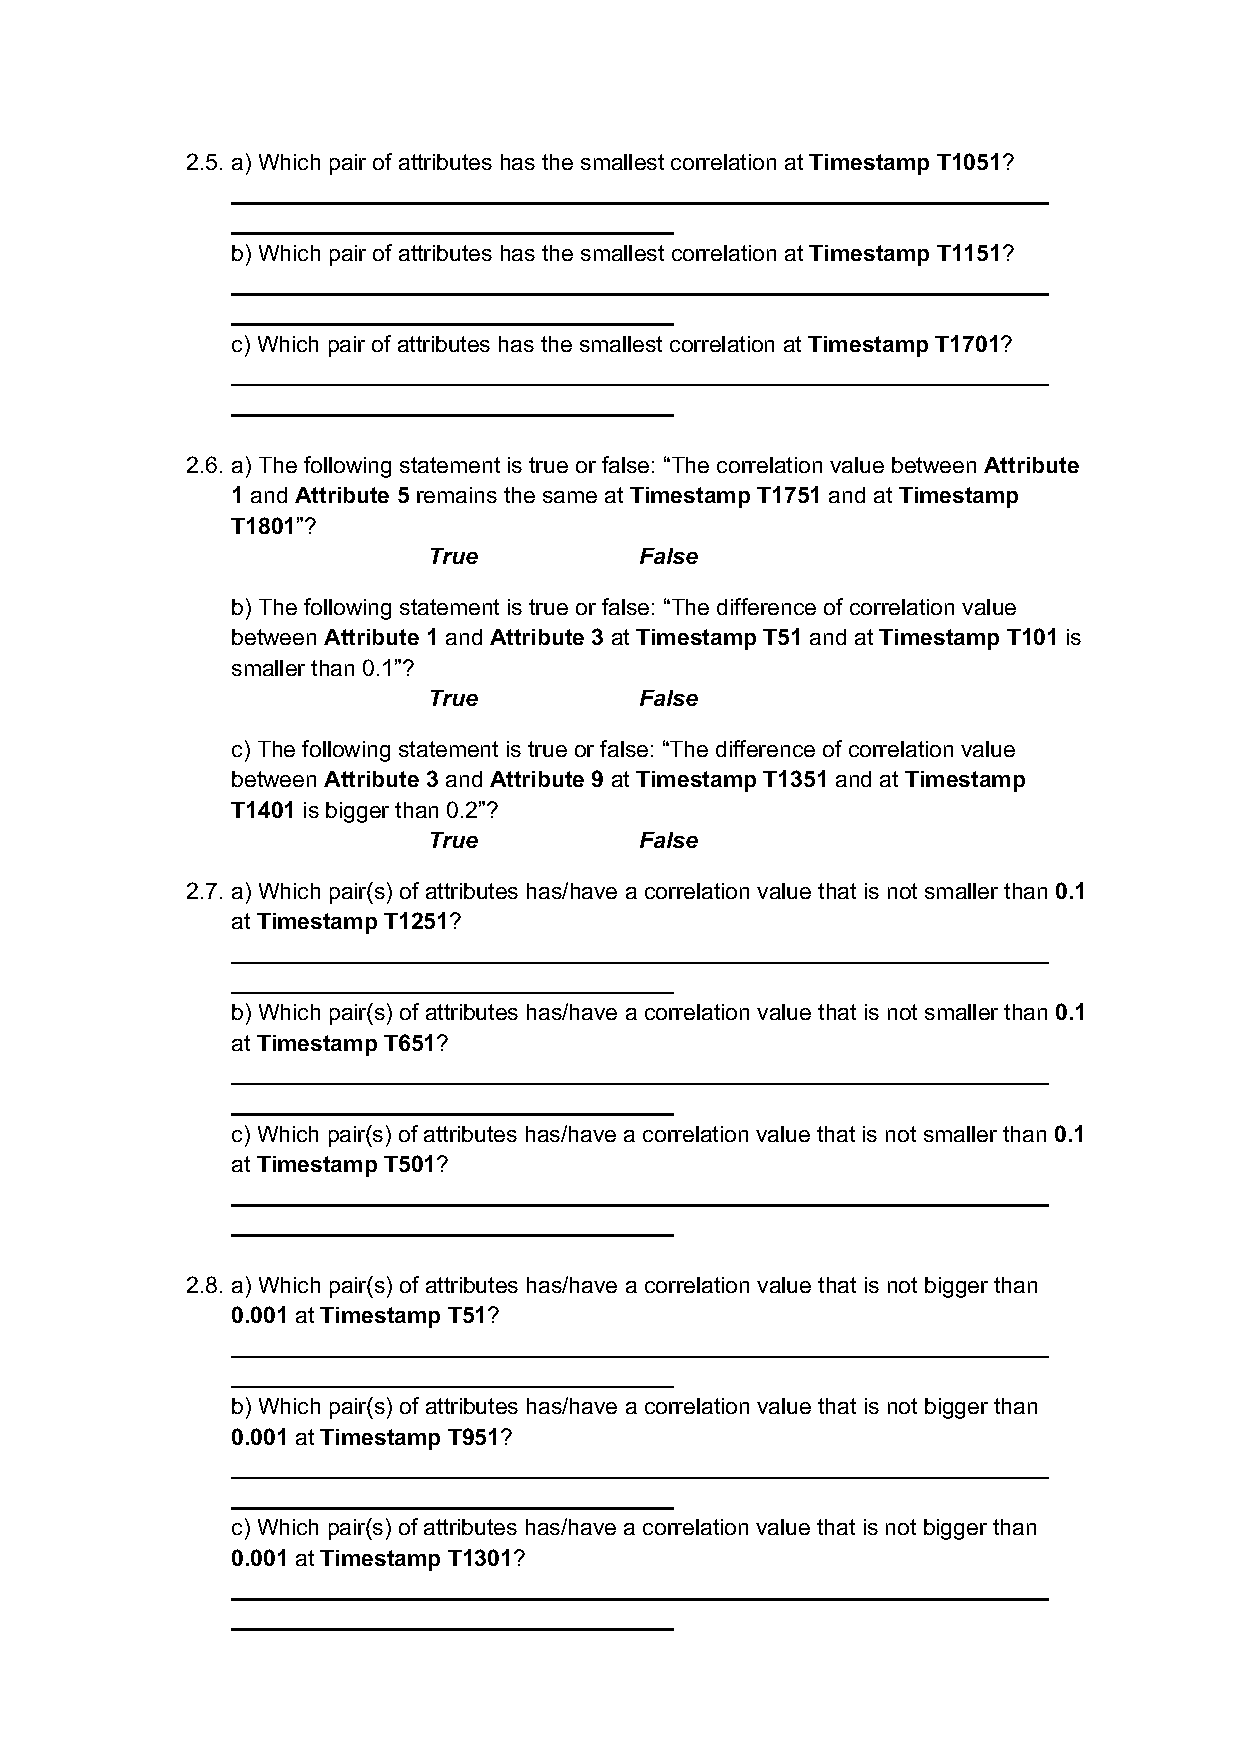
\includegraphics[scale=0.8]{us/q102.pdf}
	\newpage
	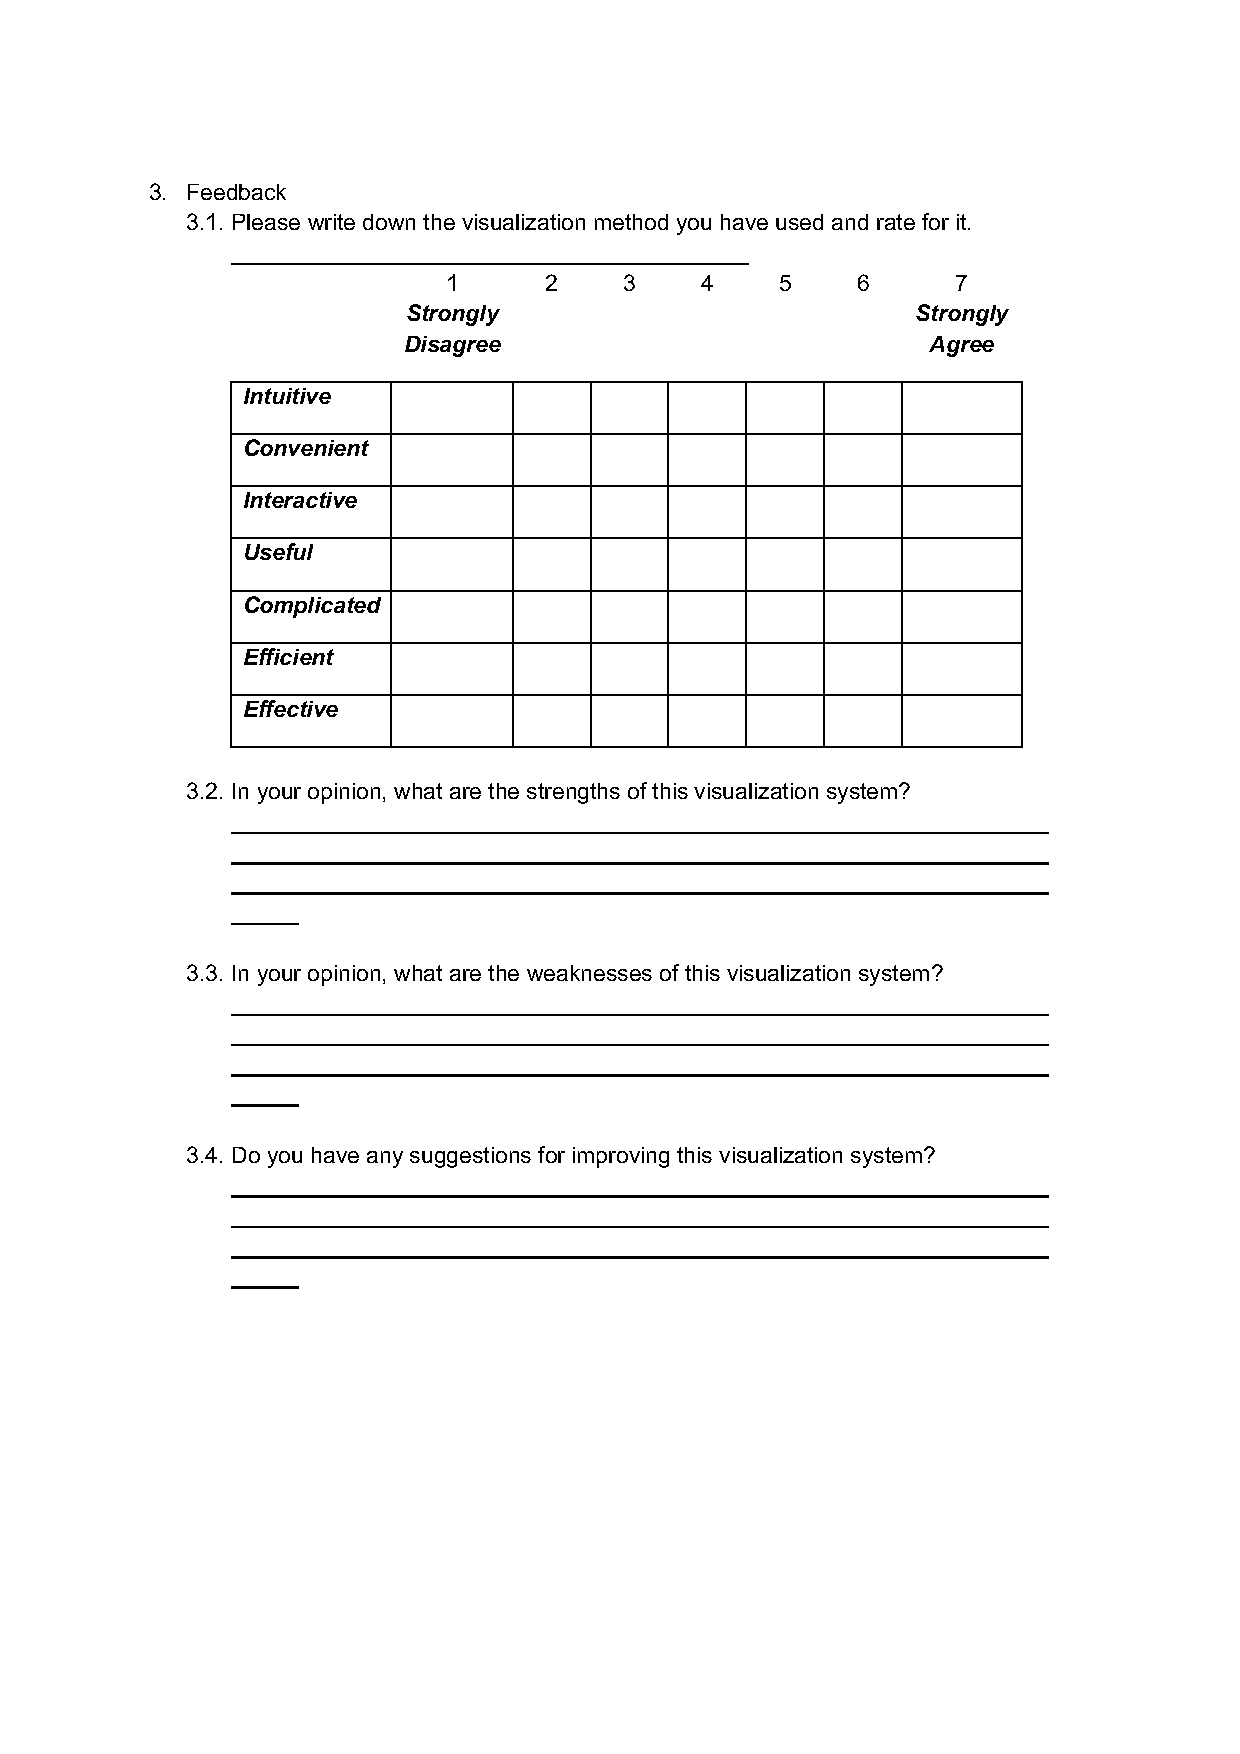
\includegraphics[scale=0.8]{us/q103.pdf}
\subsubsection{Participants using Data Set 2}
\includegraphics[scale=0.8]{us/q201.pdf}
\newpage
\includegraphics[scale=0.8]{us/q202.pdf}
\newpage
\includegraphics[scale=0.8]{us/q203.pdf}
\subsubsection{Participants using Data Set 3}
\includegraphics[scale=0.8]{us/q401.pdf}
\newpage
\includegraphics[scale=0.8]{us/q402.pdf}
\newpage
\includegraphics[scale=0.8]{us/q403.pdf}

\subsection{Questionnaire For Participants under Condition D}
\subsubsection{Participants using Data Set 1}
\includegraphics[scale=0.8]{us/q101.pdf}
\newpage
\includegraphics[scale=0.8]{us/q102.pdf}
\newpage
\includegraphics[scale=0.8]{us/D1.pdf}
\newpage
\includegraphics[scale=0.8]{us/D2.pdf}
\newpage
\includegraphics[scale=0.8]{us/D3.pdf}
\subsubsection{Participants using Data Set 2}
\includegraphics[scale=0.8]{us/q201.pdf}
\newpage
\includegraphics[scale=0.8]{us/q202.pdf}
\newpage
\includegraphics[scale=0.8]{us/D1.pdf}
\newpage
\includegraphics[scale=0.8]{us/D2.pdf}
\newpage
\includegraphics[scale=0.8]{us/D3.pdf}
\subsubsection{Participants using Data Set 3}
\includegraphics[scale=0.8]{us/q401.pdf}
\newpage
\includegraphics[scale=0.8]{us/q402.pdf}
\newpage
\includegraphics[scale=0.8]{us/D1.pdf}
\newpage
\includegraphics[scale=0.8]{us/D2.pdf}
\newpage
\includegraphics[scale=0.8]{us/D3.pdf}

%% -------------------
%% | Example content |
%% -------------------

%% ---------------------
%% | / Example content |
%% ---------------------

	
\end{document}
